 \documentclass[12pt]{article}
\usepackage[utf8]{inputenc}
\usepackage{amsmath}
\usepackage{amssymb}
\usepackage[english]{babel}
\usepackage[margin = 1 in]{geometry}
\usepackage{wrapfig}
\usepackage{enumitem}
\usepackage{caption}
\usepackage{csquotes}
\usepackage{xcolor}
\usepackage{graphicx} 
\usepackage{subfig}

\usepackage{subfig}

\title{Project 1 - SI1336 Simulation and modelling}
\author{Raymond Wang} 
\date{November 5, 2020}

\begin{document}
\maketitle
\newpage

\section*{Project 1.1}
The solutions for the position, $\theta(t)$ and velocity, $\dot{\theta}(t)$ comparisons were derived using Velocity Verlet integration. As will be shown later, this is primarily attributed to its satisfactory energy-preserving characteristics in comparison with the other methods. Initial conditions $\theta(0)/\pi = 0.1, 0.3, 0.5$ and  $\dot{\theta}(0) = 0$, in addition to a step size of $\Delta t = 0.01$ were utilized.
\subsection*{Comparisons for the harmonic oscillator}
\begin{figure*}[ht!]
\begin{center}
   \subfloat[\label{genworkflow}]{%
      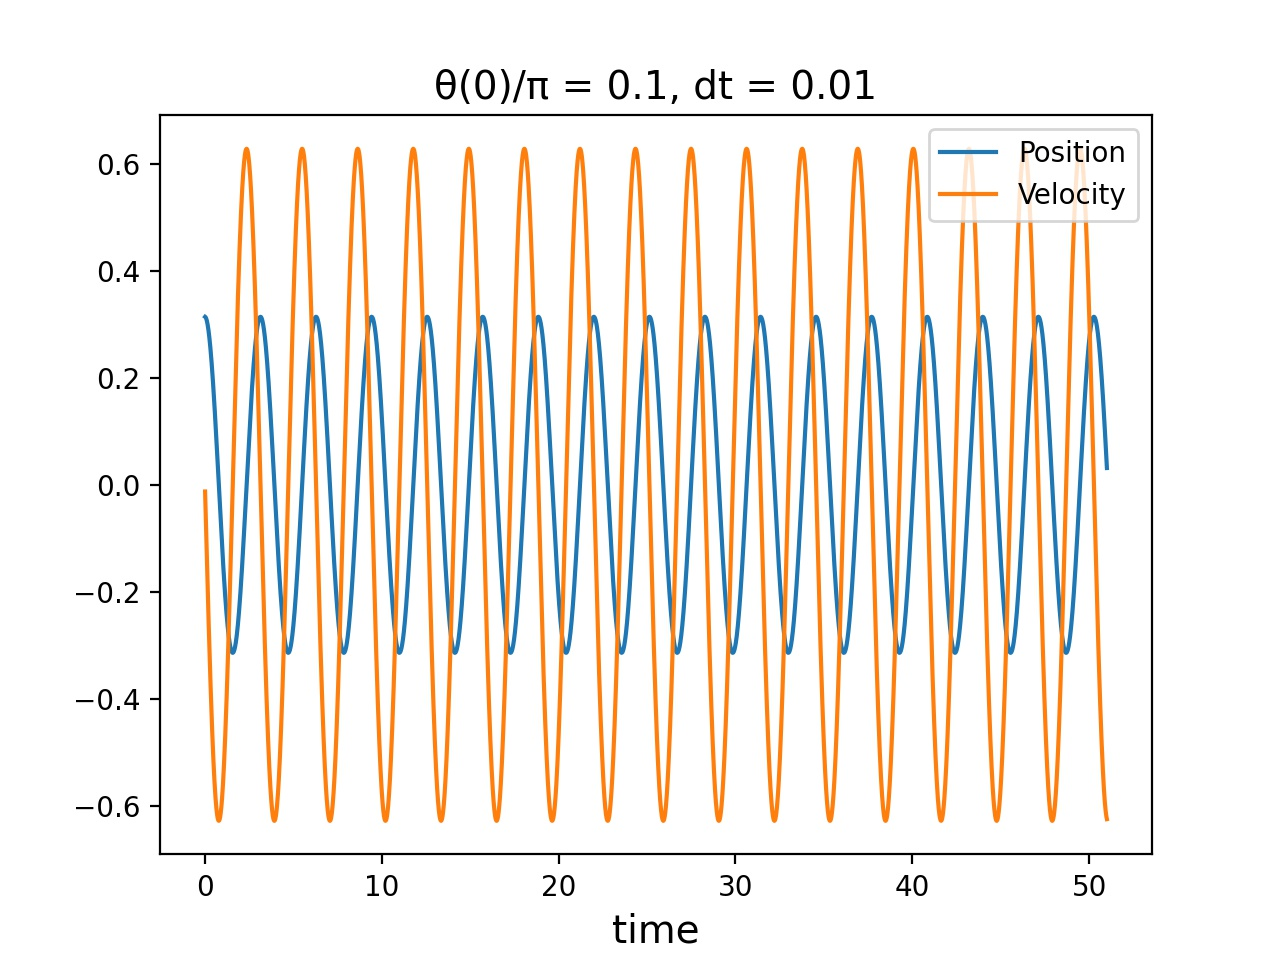
\includegraphics[width=0.33\textwidth]{Harmonic-Verlet0.1.jpg}}
   \subfloat[\label{pyramidprocess}]{%
      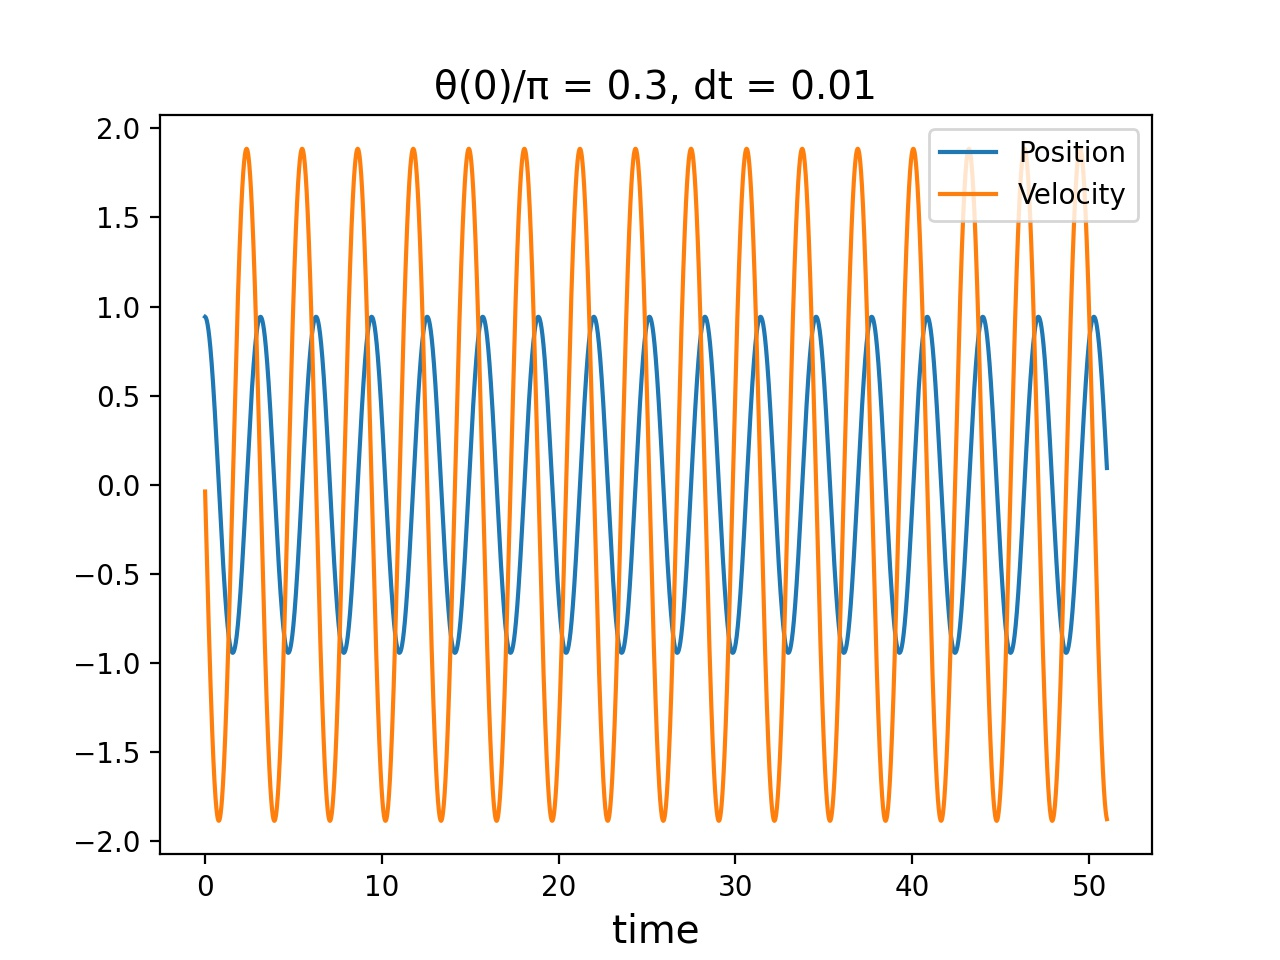
\includegraphics[ width=0.33\textwidth]{Harmonic-Verlet0.3.jpg}}
   \subfloat[\label{mt-simtask}]{%
      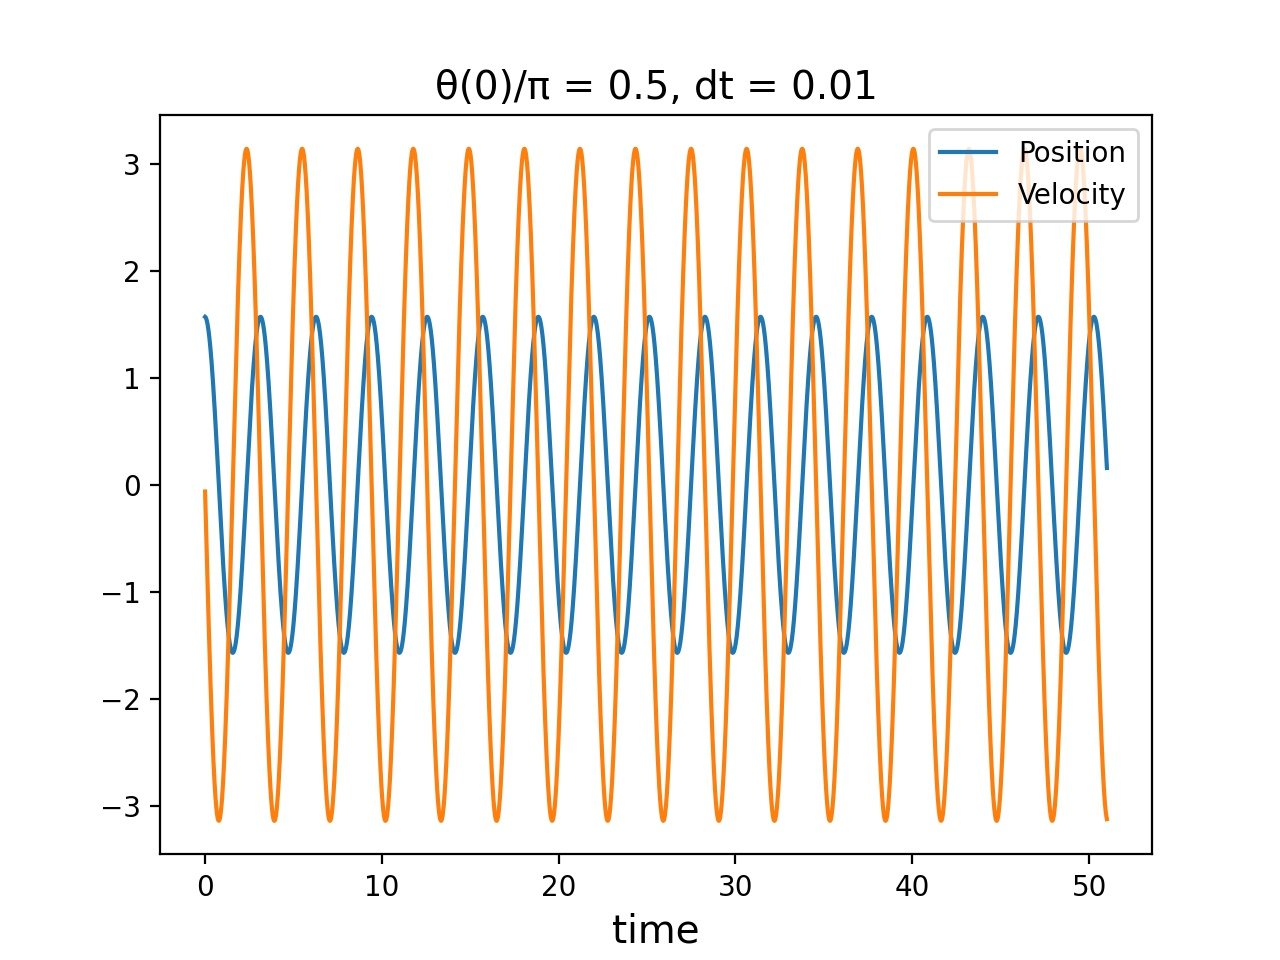
\includegraphics[ width=0.33\textwidth]{Harmonic-Verlet0.5.jpg}}\\
   \caption{\label{workflow} (a) $\theta(0)/\pi = 0.1$; (b) $\theta(0)/\pi = 0.3$; (c) $\theta(0)/\pi = 0.5$}
\end{center}
\end{figure*}

\noindent As can be noted, greater initial angle yields an increase in amplitude for the numerically simulated oscillations.
\subsection*{Comparisons for the pendulum}
\begin{figure*}[ht!]
\begin{center}
   \subfloat[\label{genworkflow}]{%
      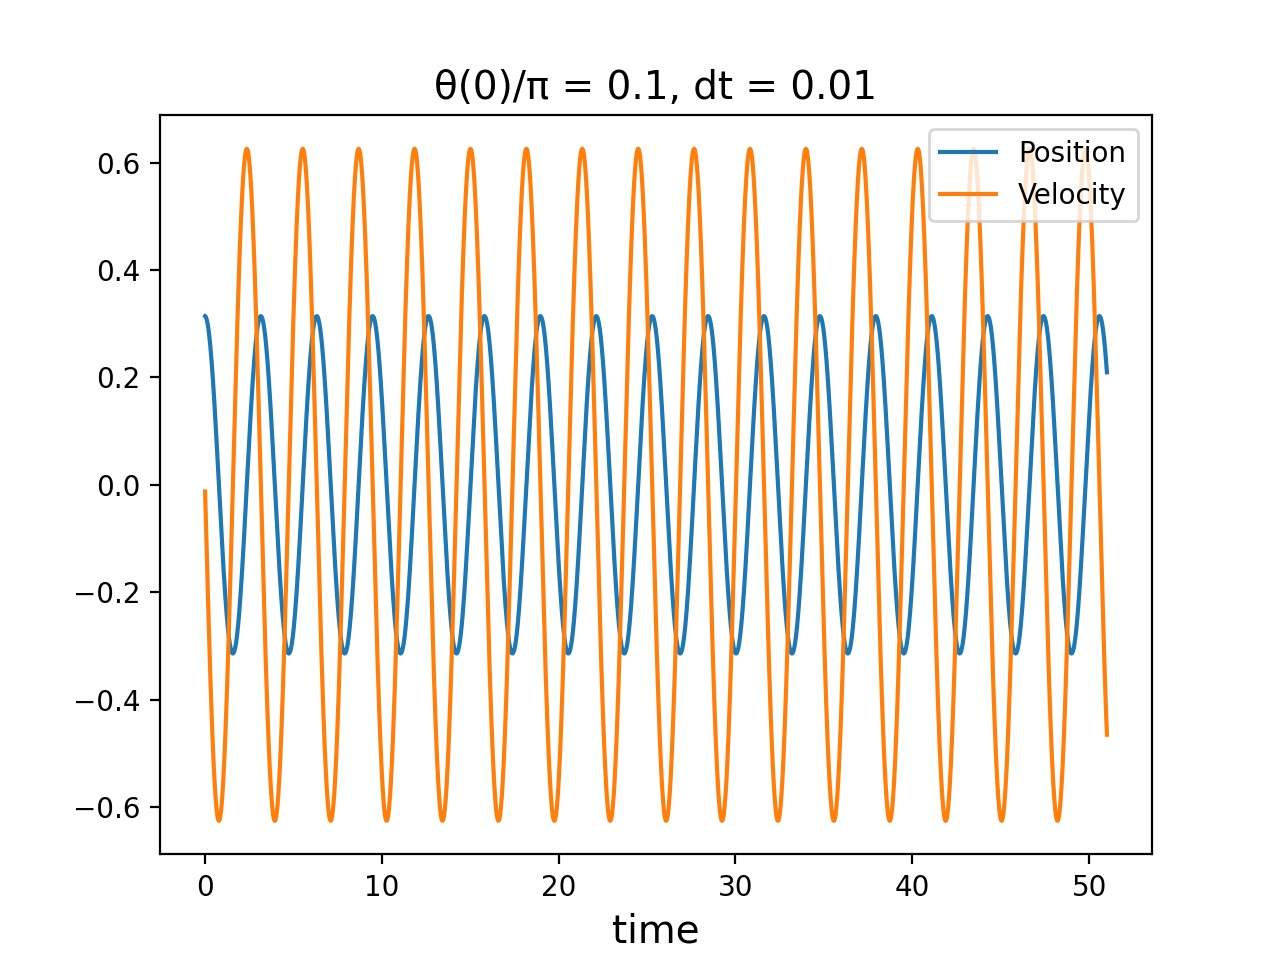
\includegraphics[ width=0.33\textwidth]{Pendulum-Verlet0.1.jpg}}
   \subfloat[\label{pyramidprocess} ]{%
      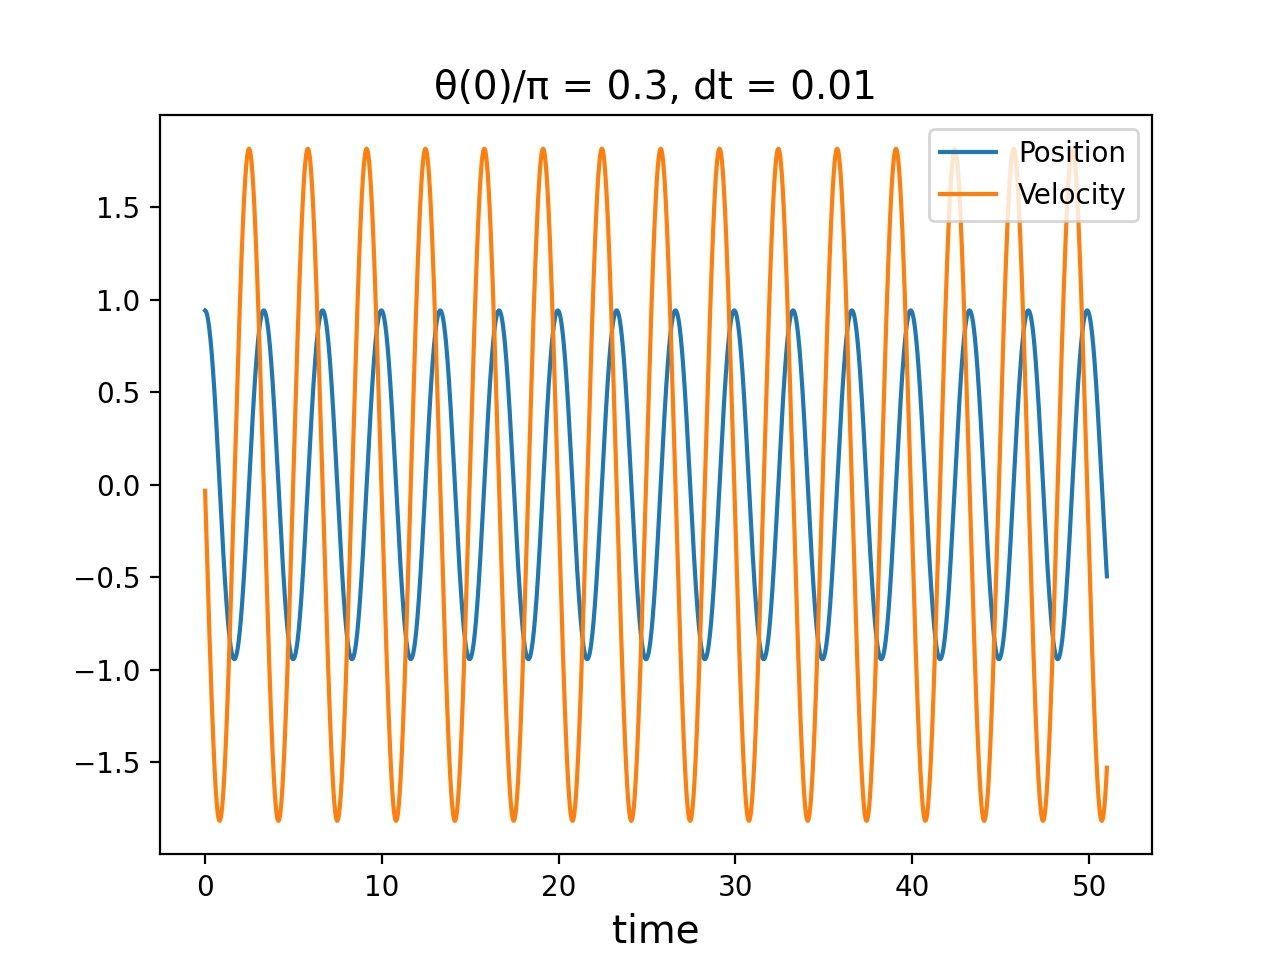
\includegraphics[ width=0.33\textwidth]{Pendulum-Verlet0.3.jpg}}
   \subfloat[\label{mt-simtask}]{%
      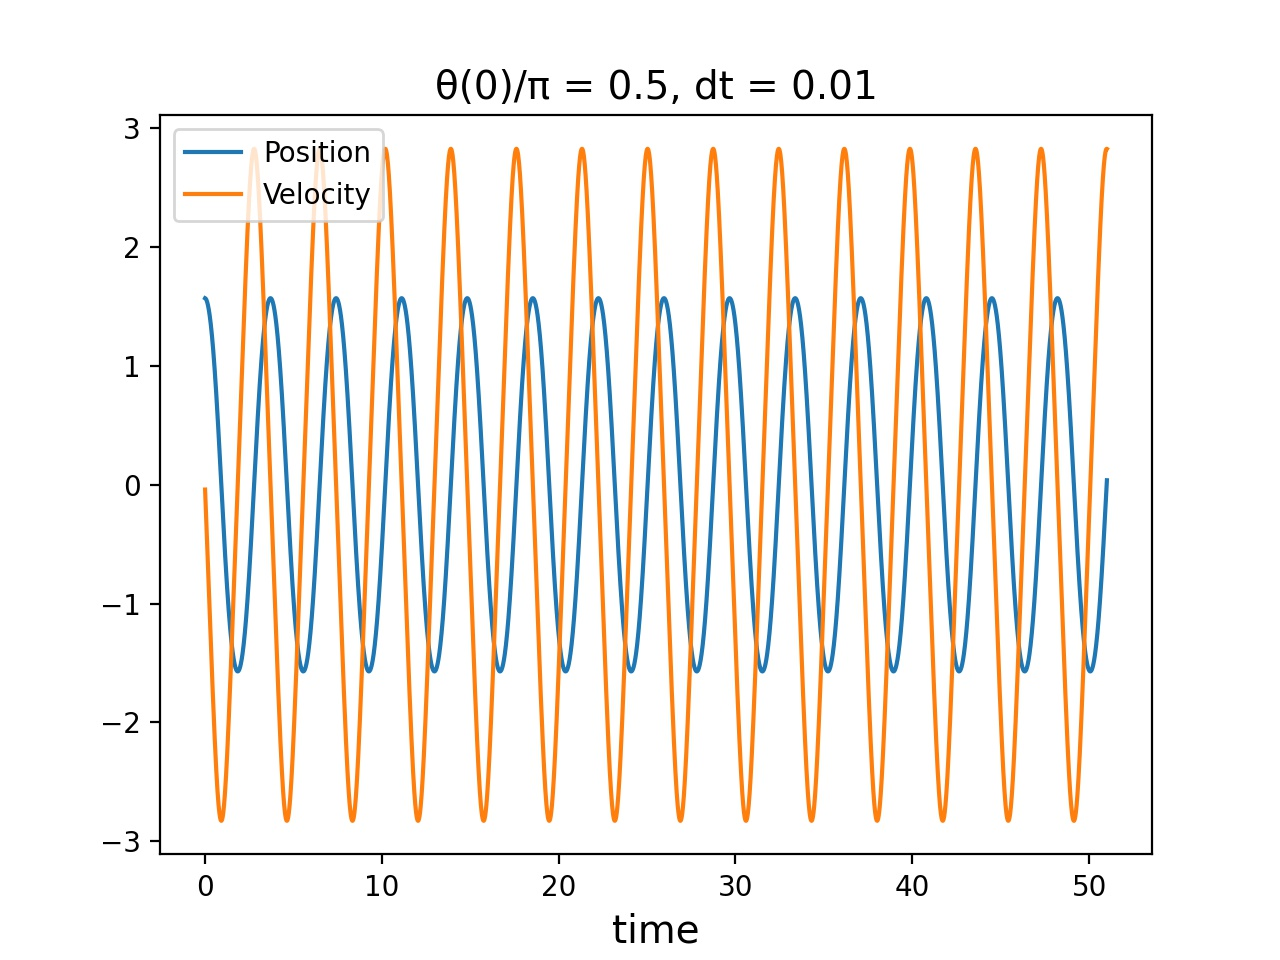
\includegraphics[ width=0.33\textwidth]{Pendulum-Verlet0.5.jpg}}\\
   \caption{\label{workflow}
   (a) $\theta(0)/\pi = 0.1$; (b) $\theta(0)/\pi = 0.3$; (c) $\theta(0)/\pi = 0.5$}
\end{center}
\end{figure*}
\noindent The simulated oscillations for the pendulum are at first glance identical to its harmonic counterpart. However, the period can be observed to be marginally shorter.

\newpage
\subsection*{Energy plots for the harmonic oscillator}
\begin{figure*}[ht!]
\begin{center}
   \subfloat[\label{genworkflow}]{%
      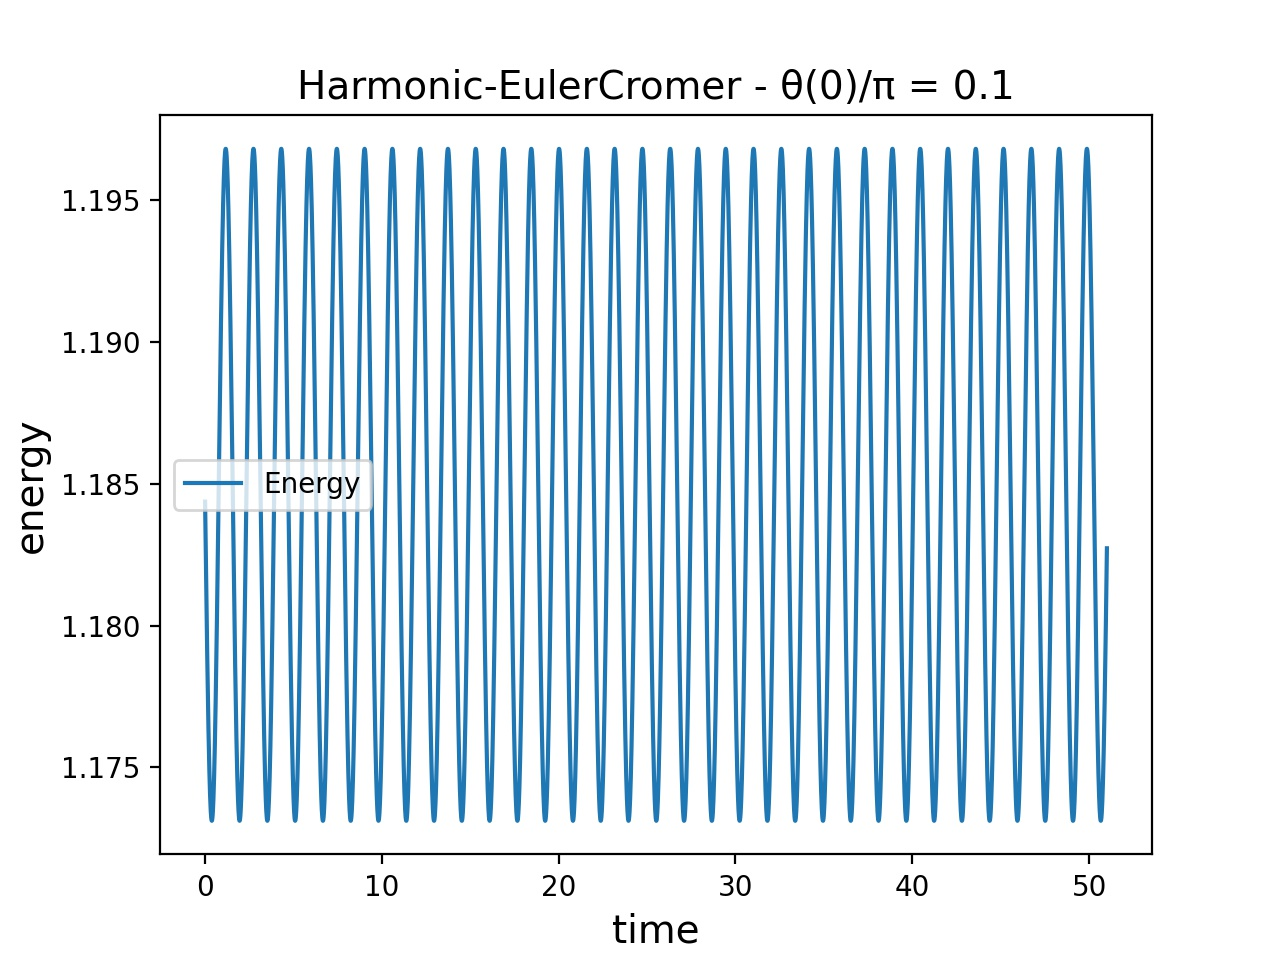
\includegraphics[ width=0.33\textwidth]{Harmonic-EulerCromer.jpg}}
   \subfloat[\label{pyramidprocess} ]{%
      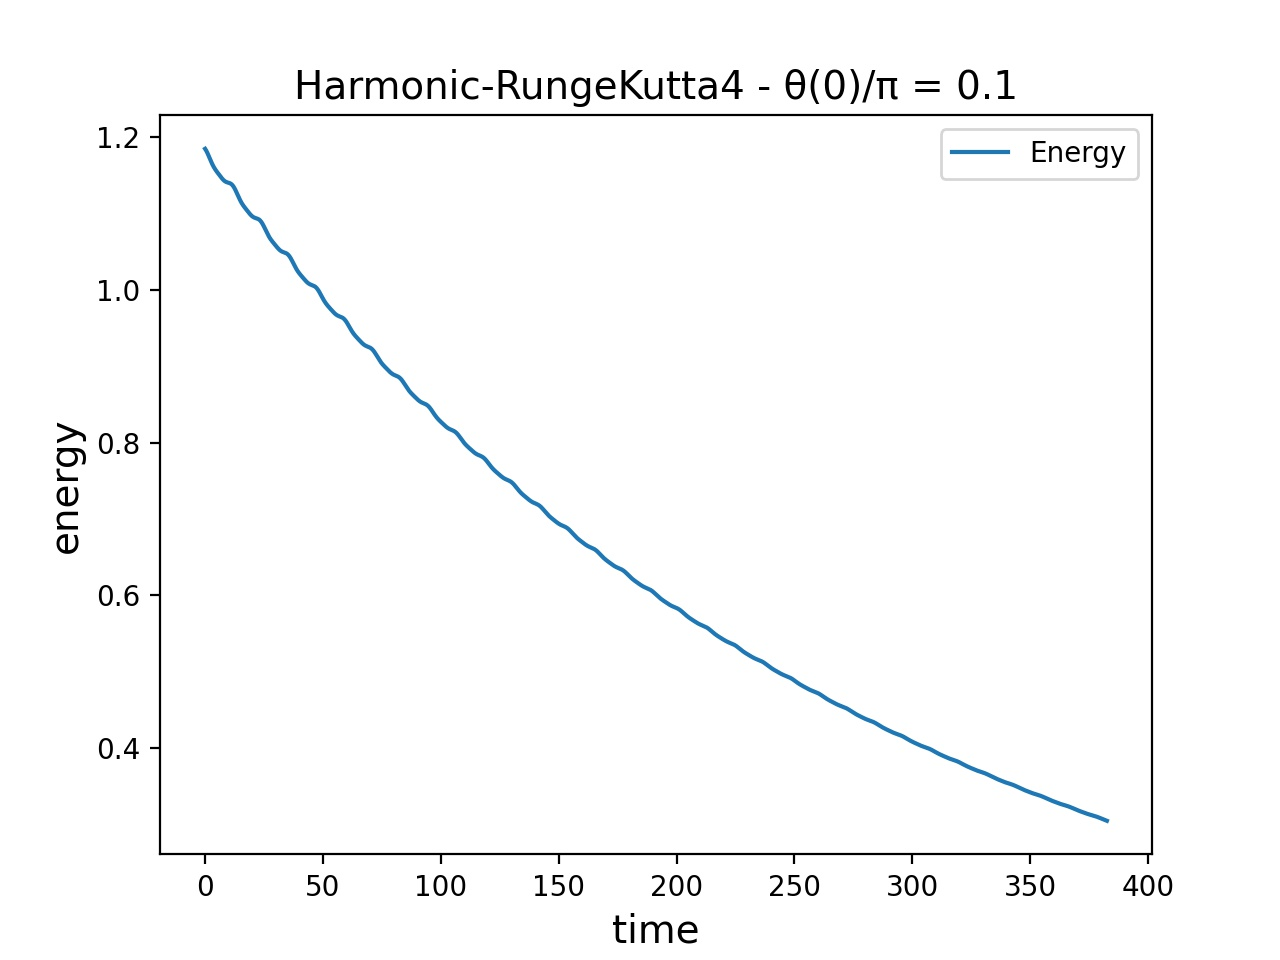
\includegraphics[ width=0.33\textwidth]{Harmonic-RungeKutta4_0.01.jpg}}
   \subfloat[\label{mt-simtask}]{%
      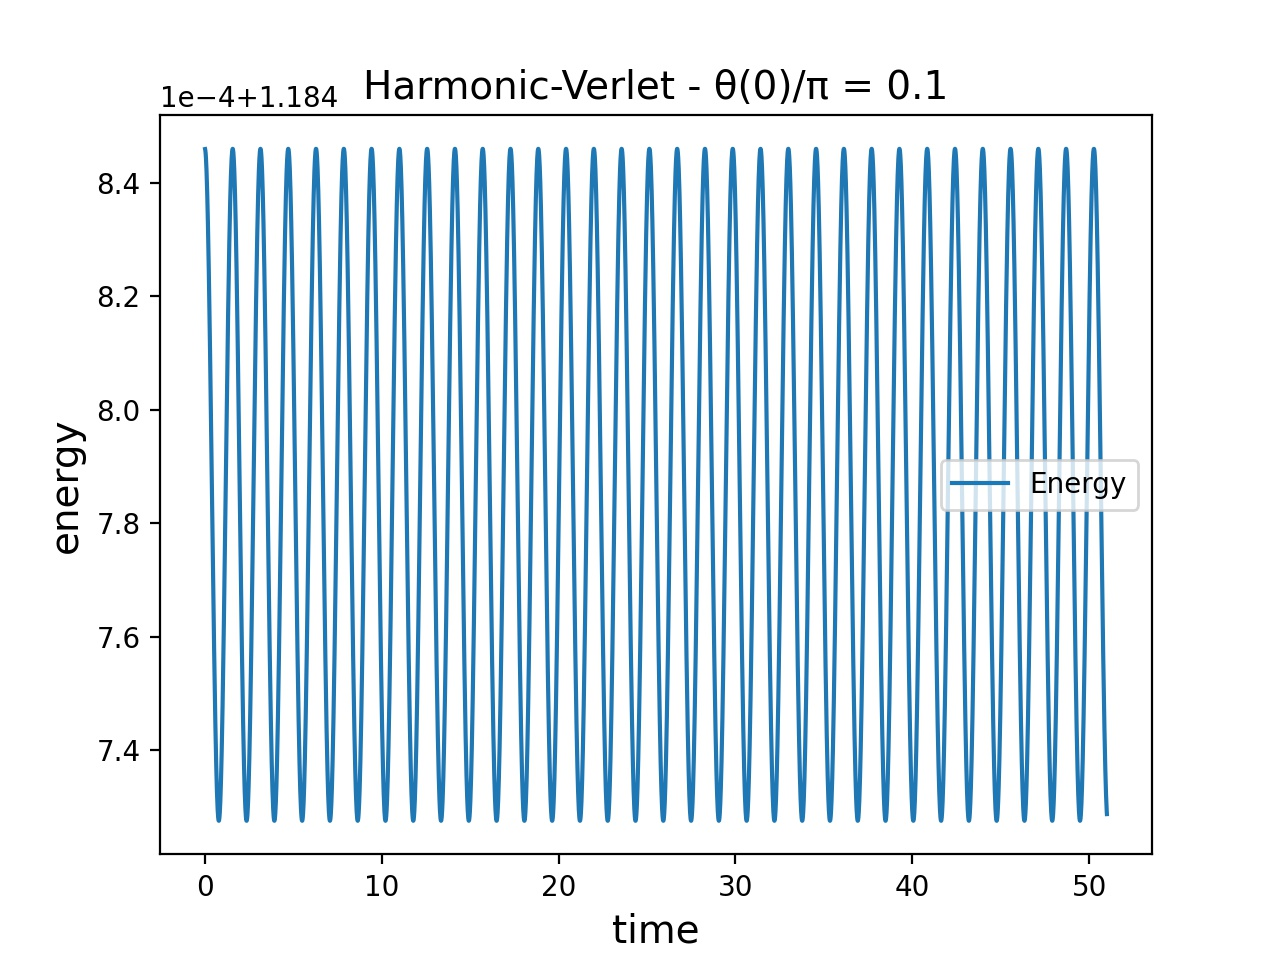
\includegraphics[ width=0.33\textwidth]{Harmonic-Verlet.jpg}}\\
   \caption{\label{workflow}. (a) Euler Cromer; 
   (b) Runge-Kutta; 
   (c) Velocity Verlet}
\end{center}
\end{figure*}
\noindent Initial conditions  $\theta(0)/\pi = 0.1$,  $\dot{\theta(0)} = 0$ and step size $\Delta t = 0.1$ were utilized for the comparison. As can be observed, the energy plots for Euler-Cromer and Velocity Verlet are sinusoidal and predominately linear for Runge-Kutta. This implies that the latter is not energy-preserving and thus  inferior as a numerical integrator. Compared to Velocity Verlet, a greater amplitude and thus energy discrepancy can be observed for Euler-Cromer. This is indicative of the satisfactory energy-preserving characteristics Velocity Verlet possesses, despite the higher order accuracy of Runge-Kutta.
\subsection*{Energy plots for the pendulum}
\begin{figure*}[ht!]
\begin{center}
   \subfloat[\label{genworkflow}]{%
      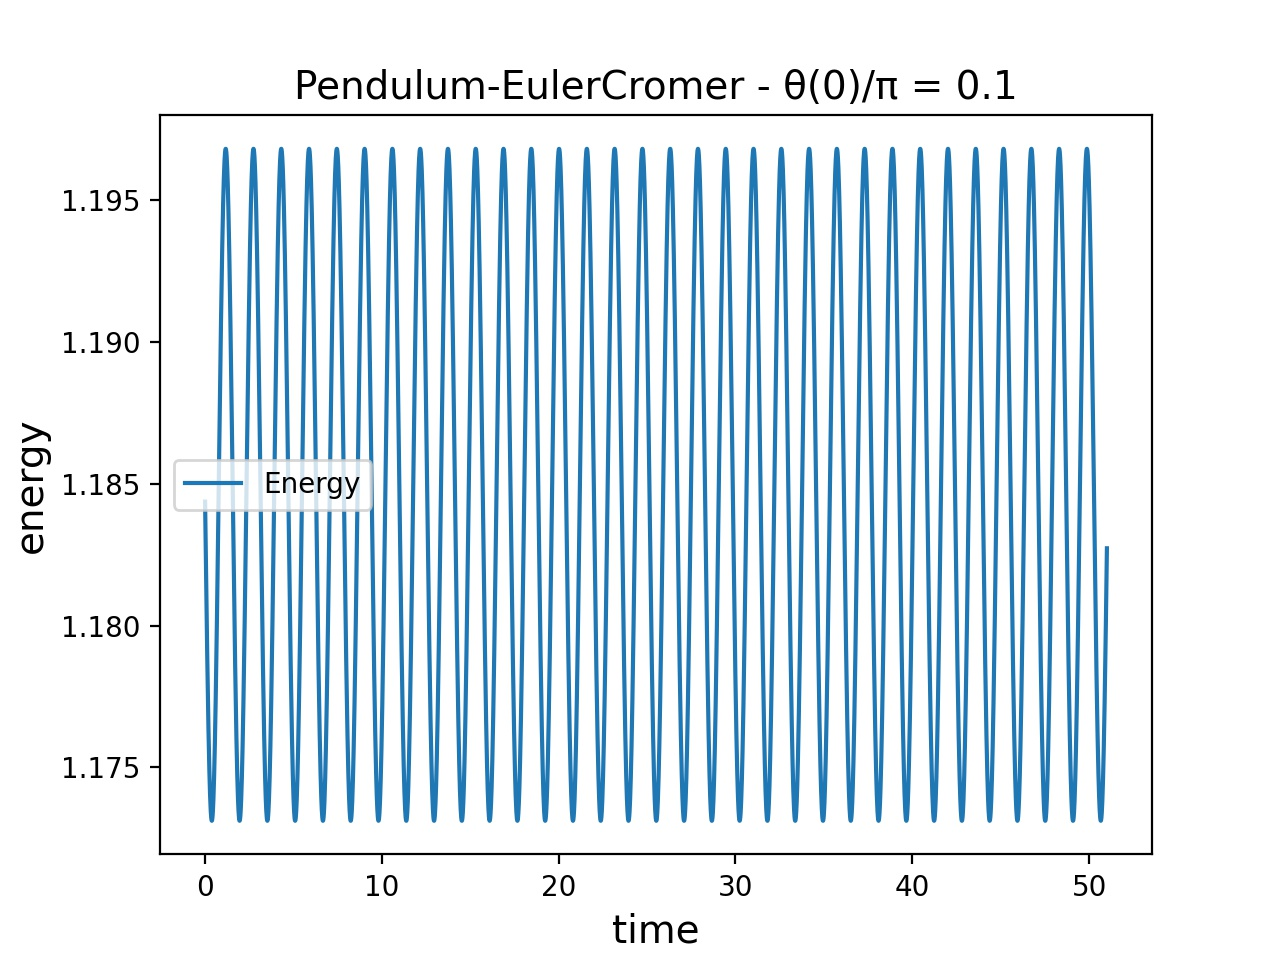
\includegraphics[ width=0.33\textwidth]{Pendulum-EulerCromer.jpg}}
   \subfloat[\label{pyramidprocess} ]{%
      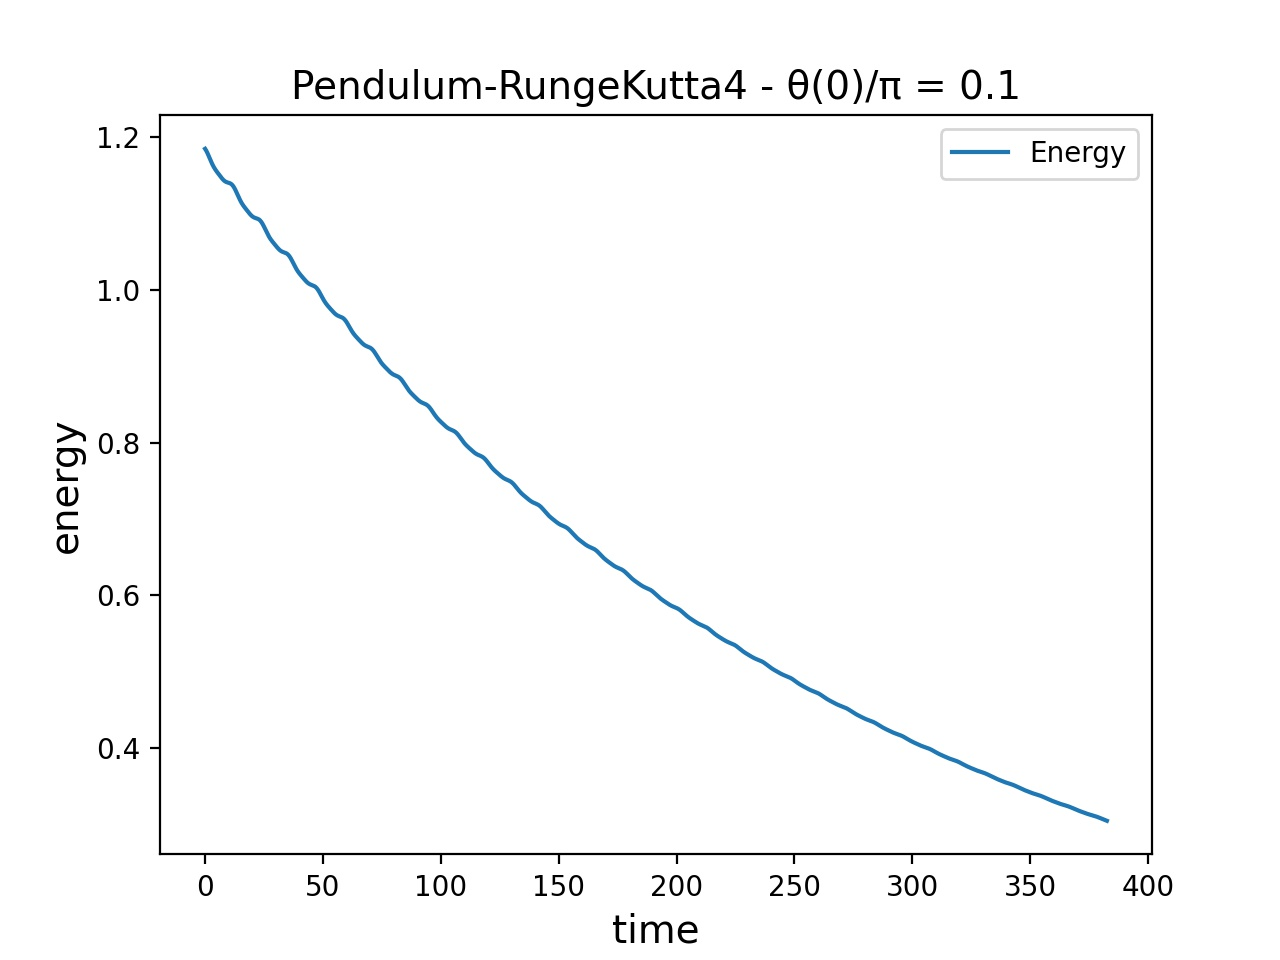
\includegraphics[ width=0.33\textwidth]{Pendulum-RungeKutta4.jpg}}
   \subfloat[\label{mt-simtask}]{%
      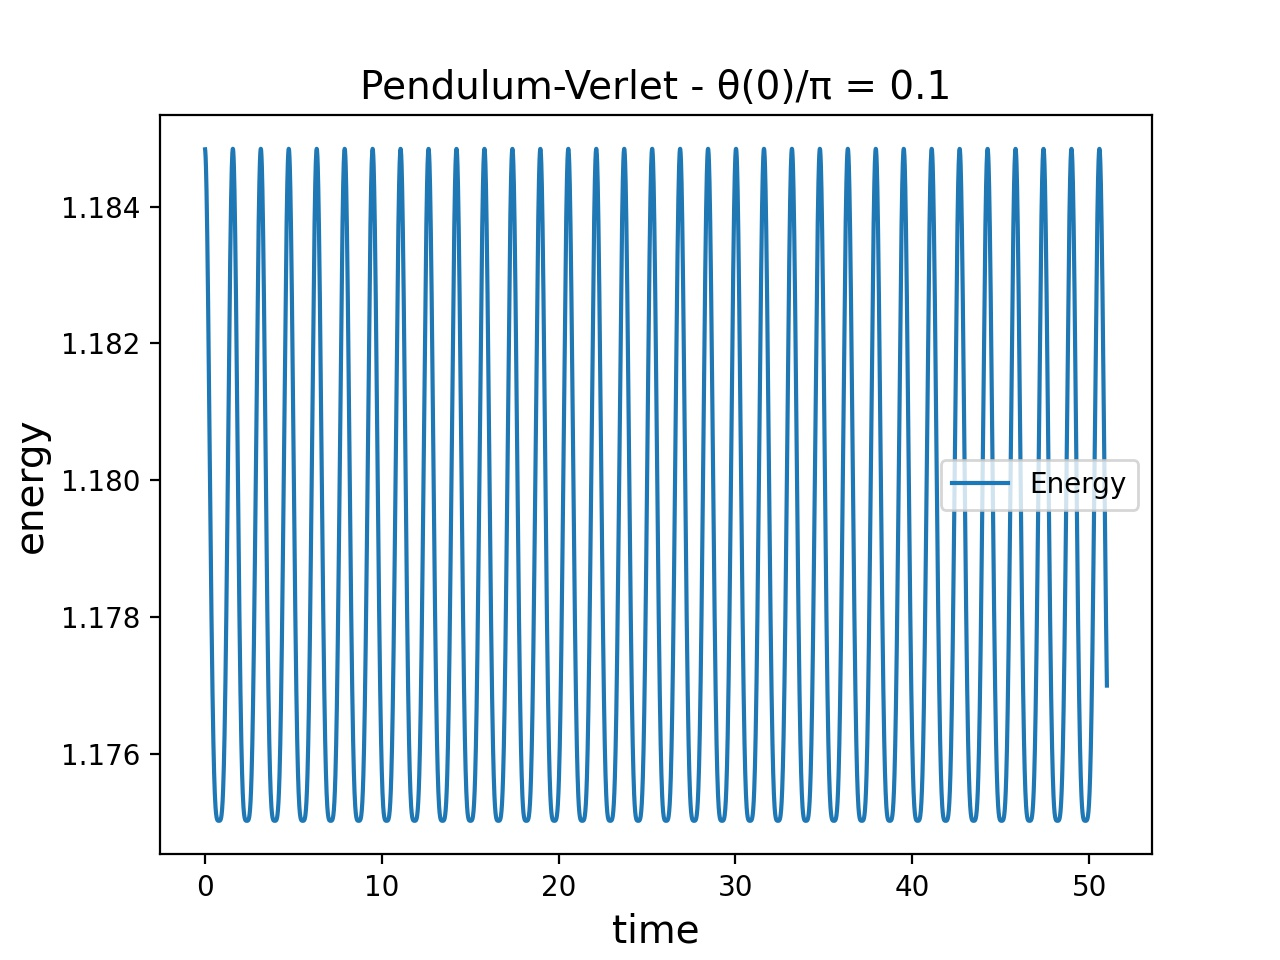
\includegraphics[ width=0.33\textwidth]{Pendulum-Verlet.jpg}}\\
   \caption{\label{workflow}
   (a) Euler Cromer; 
   (b) Runge-Kutta; 
   (c) Velocity Verlet}
\end{center}
\end{figure*}
\noindent The energy plots for the pendulum are similar compared to the harmonic oscillator, although Runge-Kutta demonstrates a more sinusoidal behavior with greater variance. 
It can also be noted that Velocity Verlet works  inferiorly due to a much greater amplitude as compared to the harmonic oscillator.

\newpage
\subsection*{Comparison of different step sizes for Runge-Kutta}
\begin{figure*}[ht!]
\begin{center}
   \subfloat[\label{genworkflow}]{%
      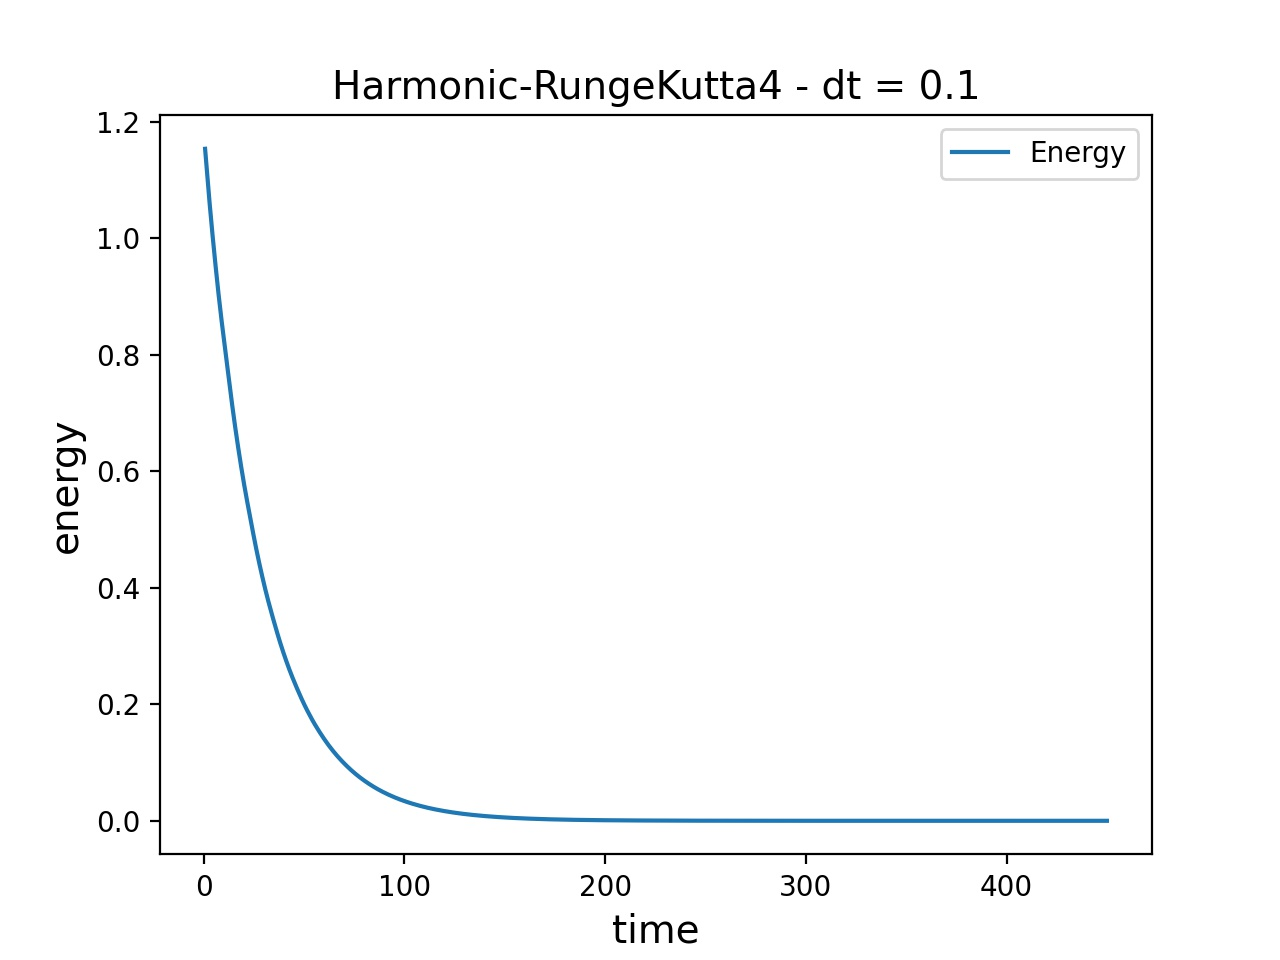
\includegraphics[ width=0.33\textwidth]{Harmonic-RungeKutta4_0.1.jpg}}
   \subfloat[\label{pyramidprocess} ]{%
      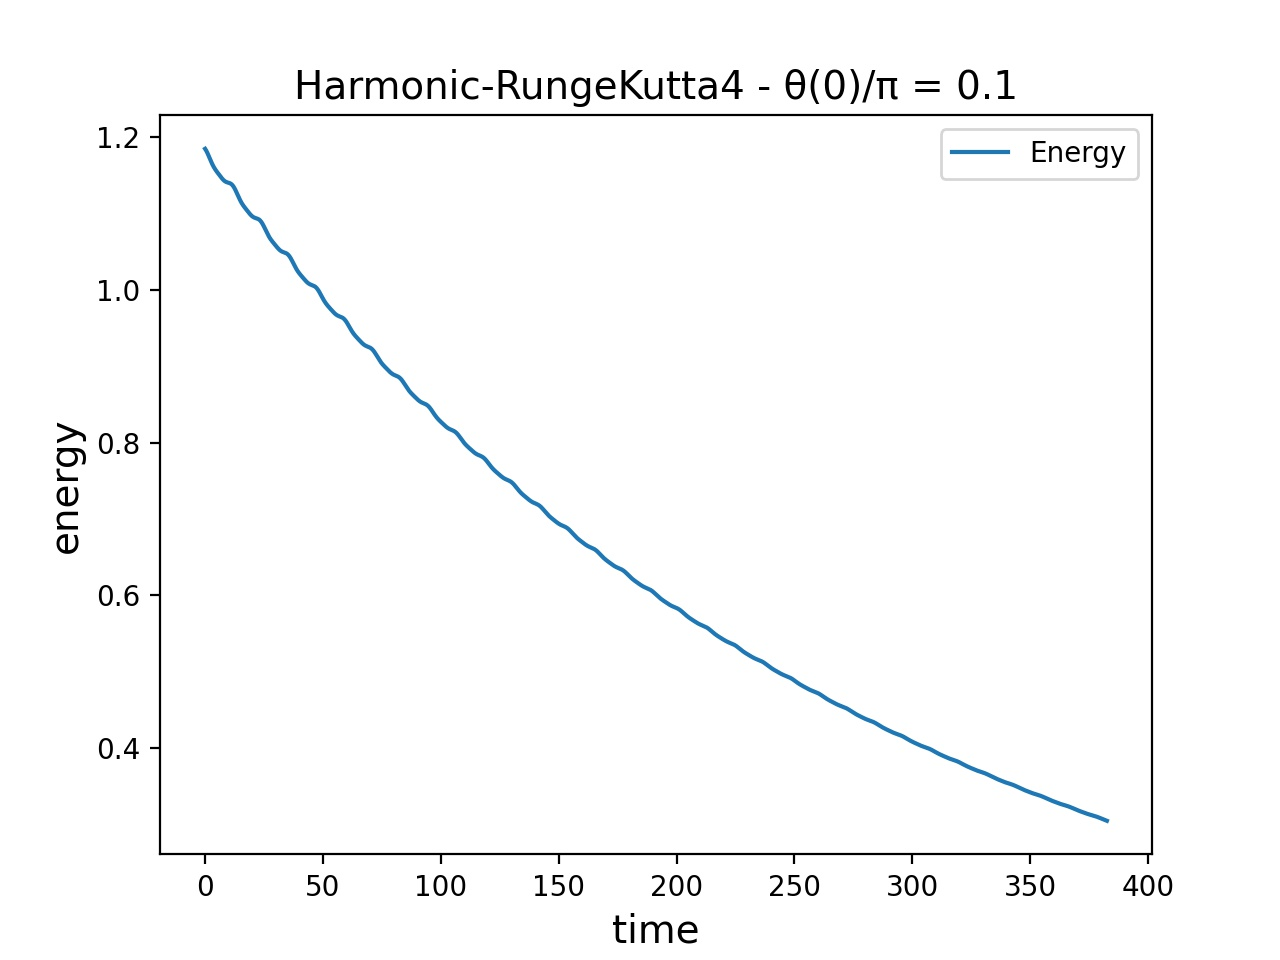
\includegraphics[ width=0.33\textwidth]{Harmonic-RungeKutta4_0.01.jpg}}
   \subfloat[\label{mt-simtask}]{%
      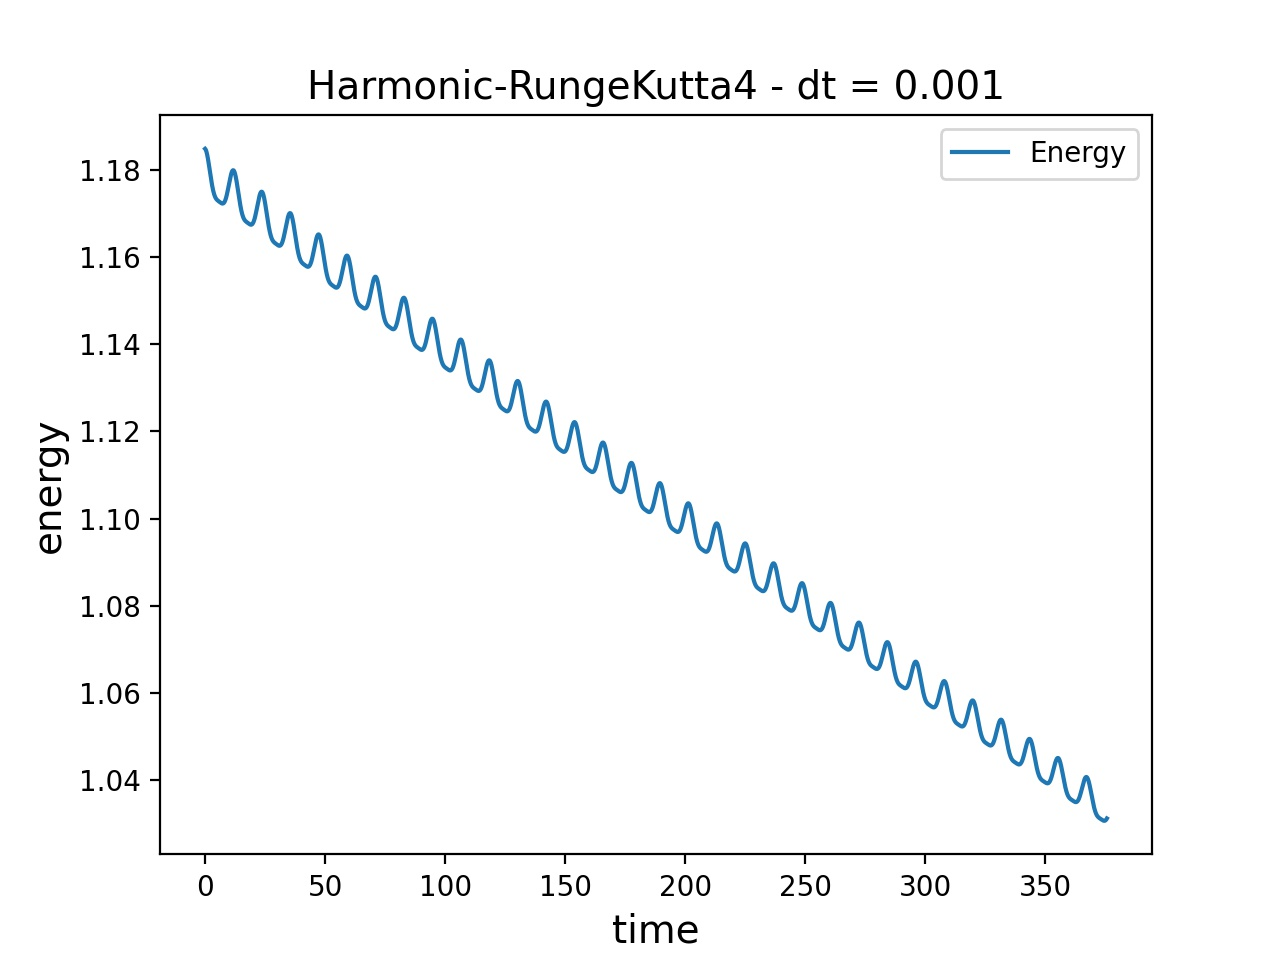
\includegraphics[ width=0.33\textwidth]{Harmonic-RungeKutta4_0.001.jpg}}\\
   \caption{\label{workflow}
   (a) $ \Delta t = 0.1$; 
   (b) $ \Delta t = 0.01$; 
   (c) $\Delta t = 0.001$}
\end{center}
\end{figure*}
\noindent In the order of 50 seconds, Runge-Kutta starts demonstrating a satisfactory linear behavior for a time step of $\Delta t = 0.1$ and $\Delta t = 0.01$ while becoming exponential for $\Delta t = 0.1$. Longer times require more marginal $t$ in order to yield adequate results.
\subsection*{Harmonic oscillator - Analytical and numerical solution}
\begin{figure*}[ht!]
\begin{center}
    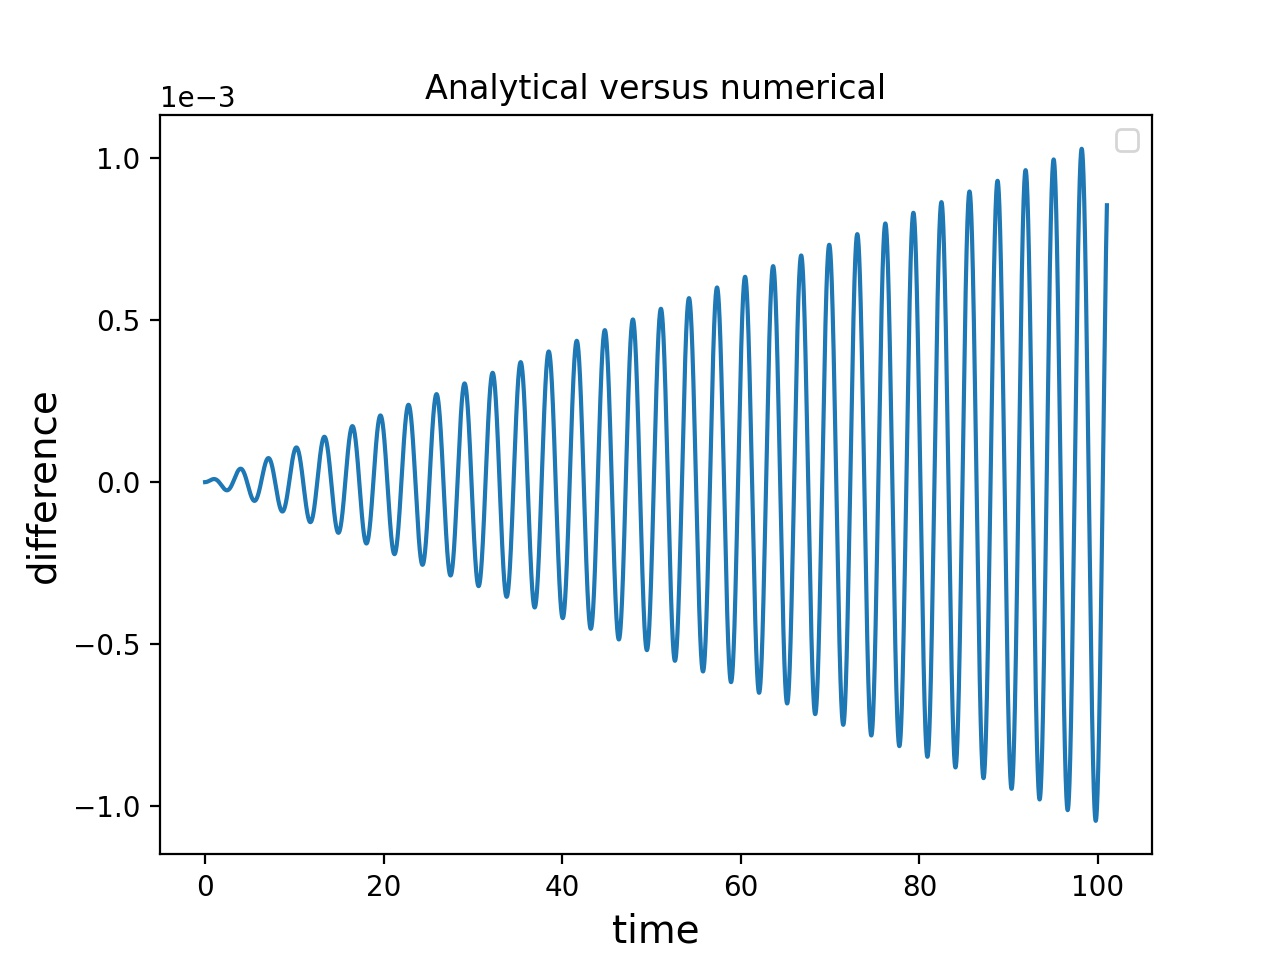
\includegraphics[ width=0.45\textwidth]{Analytical-Numerical.jpg}
 \caption{}
\end{center}
\end{figure*}
\noindent Using Verlet integration, 
$\theta(0)/\pi = 0$ and $\Delta t = 0.1$ the above-mentioned behavior are to be observed.
The difference between the analytical and numerical solutions are calculated as: 
\begin{equation*}
\text{analytical}(t) - \text{numerical}(t),
\end{equation*}
where:
\begin{equation*}
\text{analytical}(t) 
= \theta(0)\pi\cdot\text{cos}(\sqrt{g/l}\cdot t) 
\end{equation*}
Since the the discrepancy is within the order of $10^{-3}$. it can be concluded that the numerical solutions are of high precision.


\newpage
\section*{Project 1.2}
\subsection*{Comparison between the pendulum and perturbation series}
\begin{figure*}[ht!]
\begin{center}
    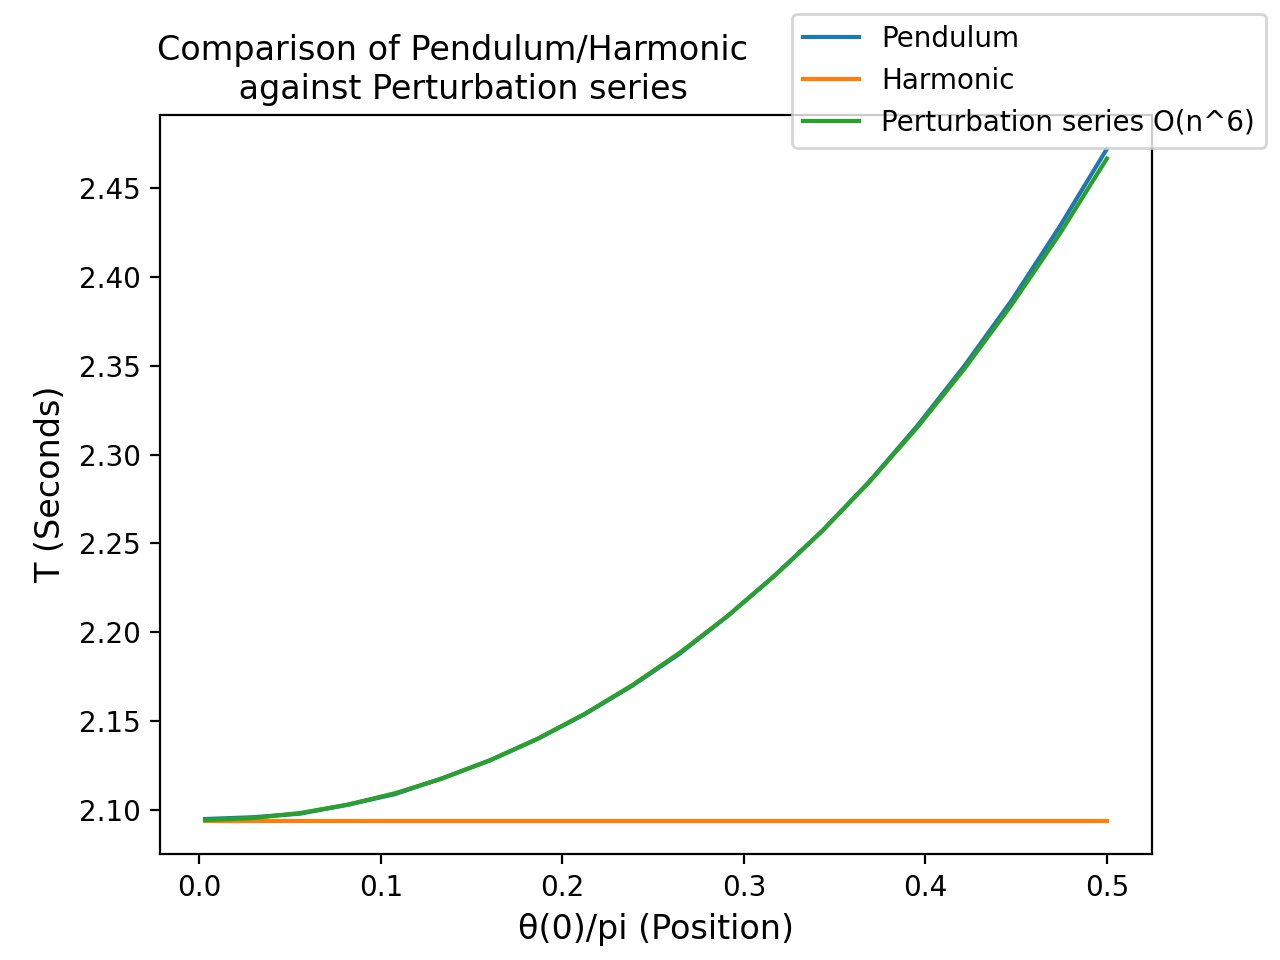
\includegraphics[width=0.5\textwidth]{Perturbation.png}
 \caption{}
\end{center}
\end{figure*}
\noindent The sixth power of the perturbation series, i.e:
\begin{equation*}
T = 2\pi\sqrt{\cfrac{l}{g}}\bigg(1 + \cfrac{1}{16}\text{ }\theta^2(0) + \cfrac{11}{3072}\text{ }\theta^4(0) + \cfrac{173}{737280}\text{ }\theta^6(0)\bigg),  
\end{equation*}
\noindent sufficiently approximates the exponentially increasing period of the pendulum, while the period of the harmonic oscillator remains constant.

\newpage
\section*{Project 1.3}
\subsection*{The dampened harmonic oscillator}
\begin{figure*}[ht!]
\begin{center}
   \subfloat[\label{genworkflow}]{%
      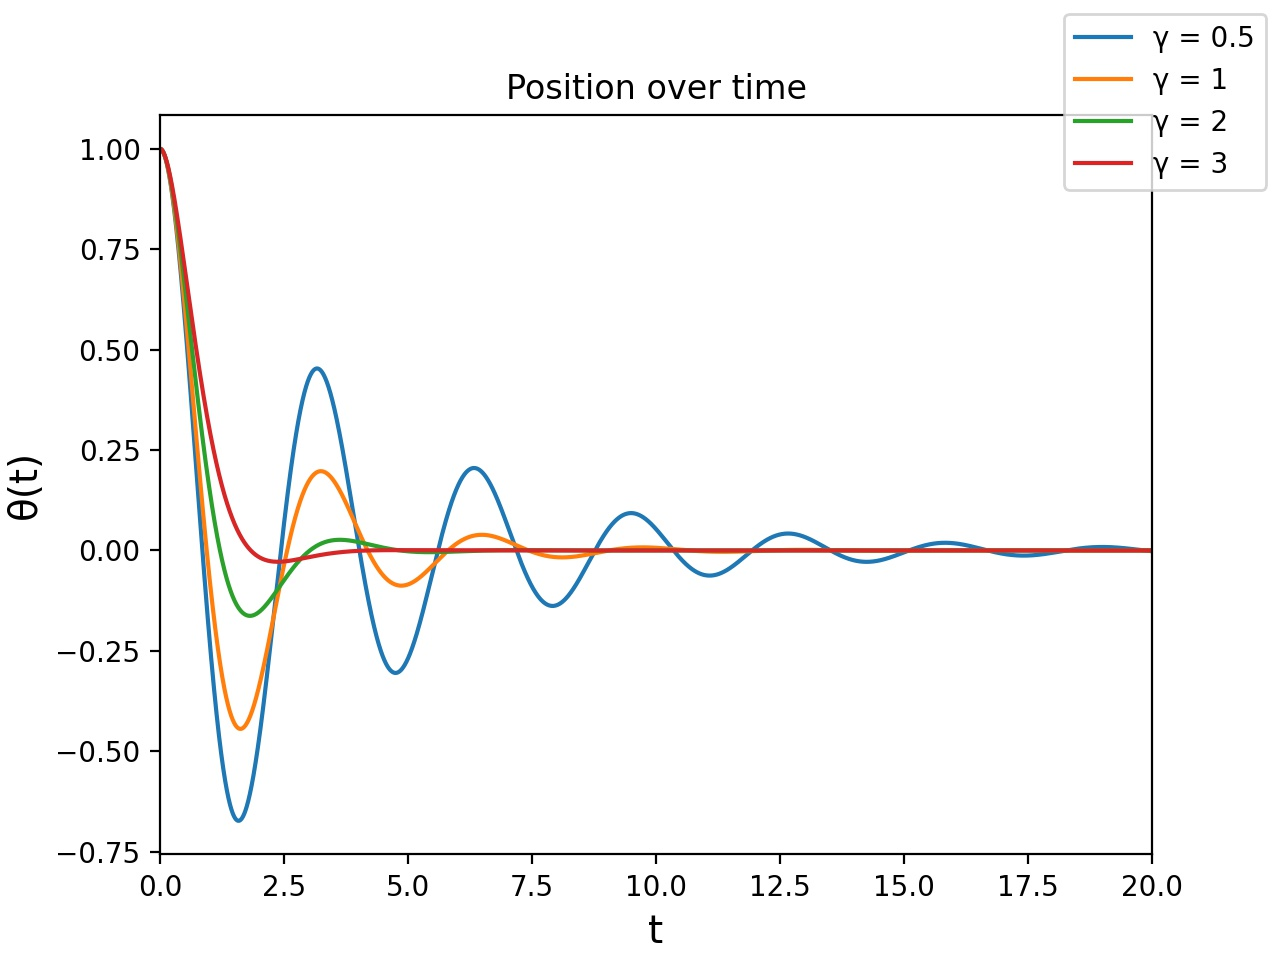
\includegraphics[ width=0.33\textwidth]{Position.jpg}}
   \subfloat[\label{pyramidprocess} ]{%
      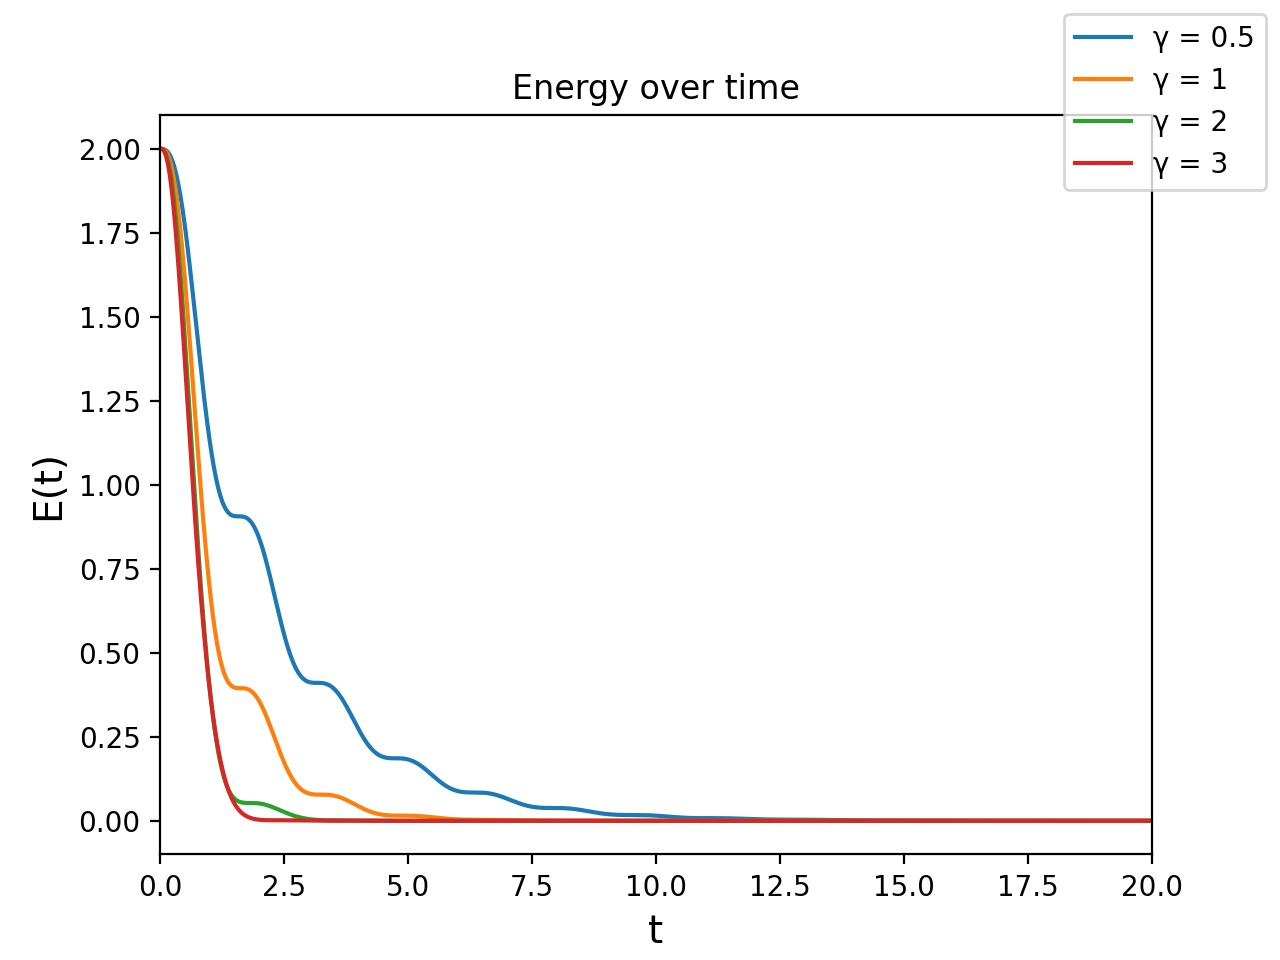
\includegraphics[ width=0.33\textwidth]{Energy.jpg}}
   \subfloat[\label{mt-simtask}]{%
      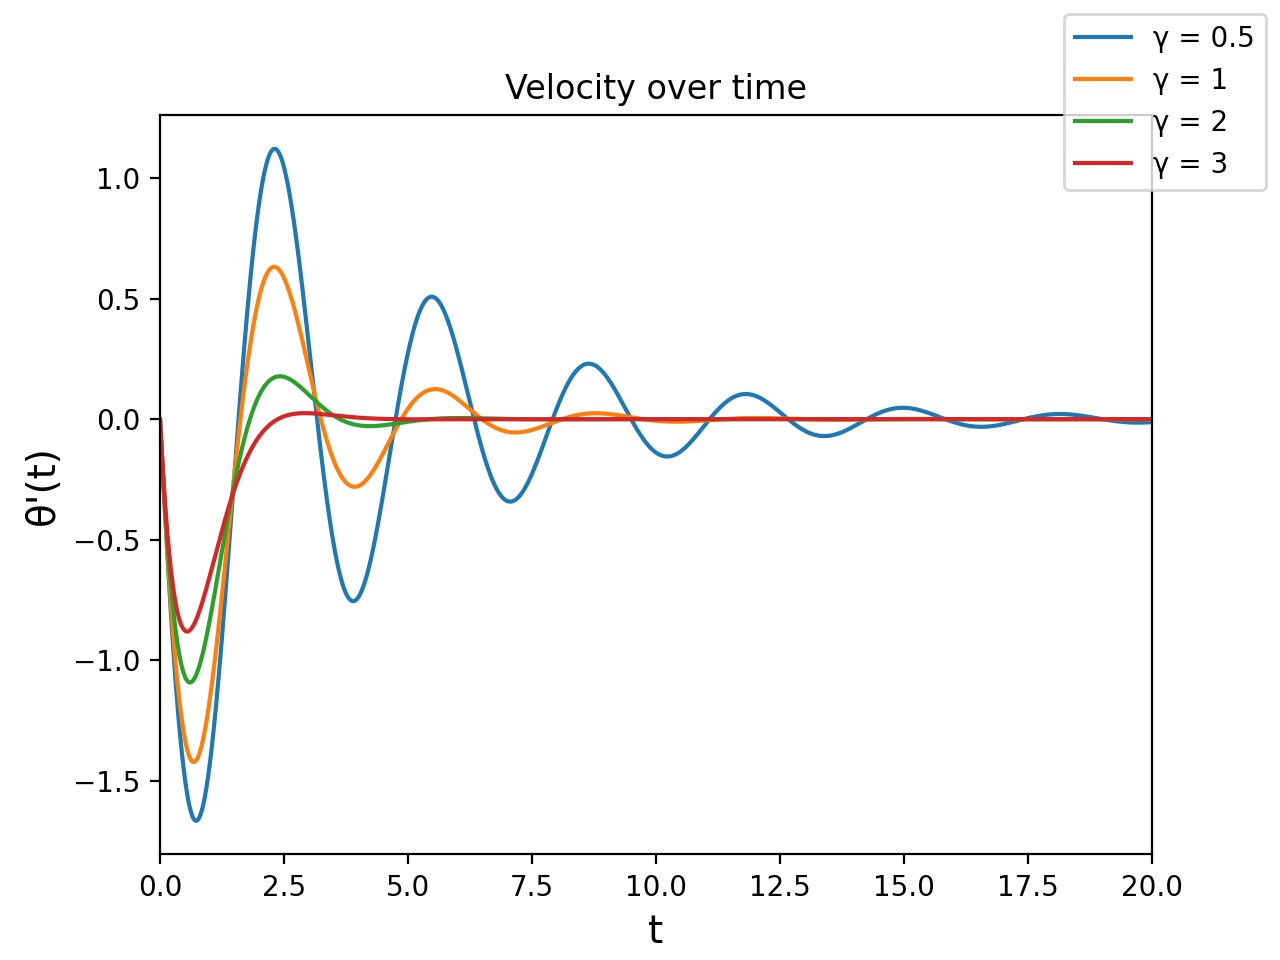
\includegraphics[ width=0.33\textwidth]{Velocity.jpg}}\\
   \caption{\label{workflow} (a) Position over time; 
   (b) Energy over time; 
   (c) Velocity over time.}
\end{center}
\end{figure*}
\noindent $\bullet$ Plot (a) Greater values for $\gamma$ result in a decrease the relaxation time 
\vspace{0.2cm}
\newline
\noindent $\bullet$ Plot (b) Energy decreases over time. Greater values for $\gamma$ amplify the reduction speed.
\vspace{0.2cm}
\newline
\noindent $\bullet$ Plot (c) Greater values for $\gamma$ result in a decrease of the relaxation time. 
\newline 
\textcolor{white}o It can also be noted that the velocity decreases over time.

\subsection*{Relaxation time over $\gamma$}
\begin{figure*}[ht!]
\begin{center}
    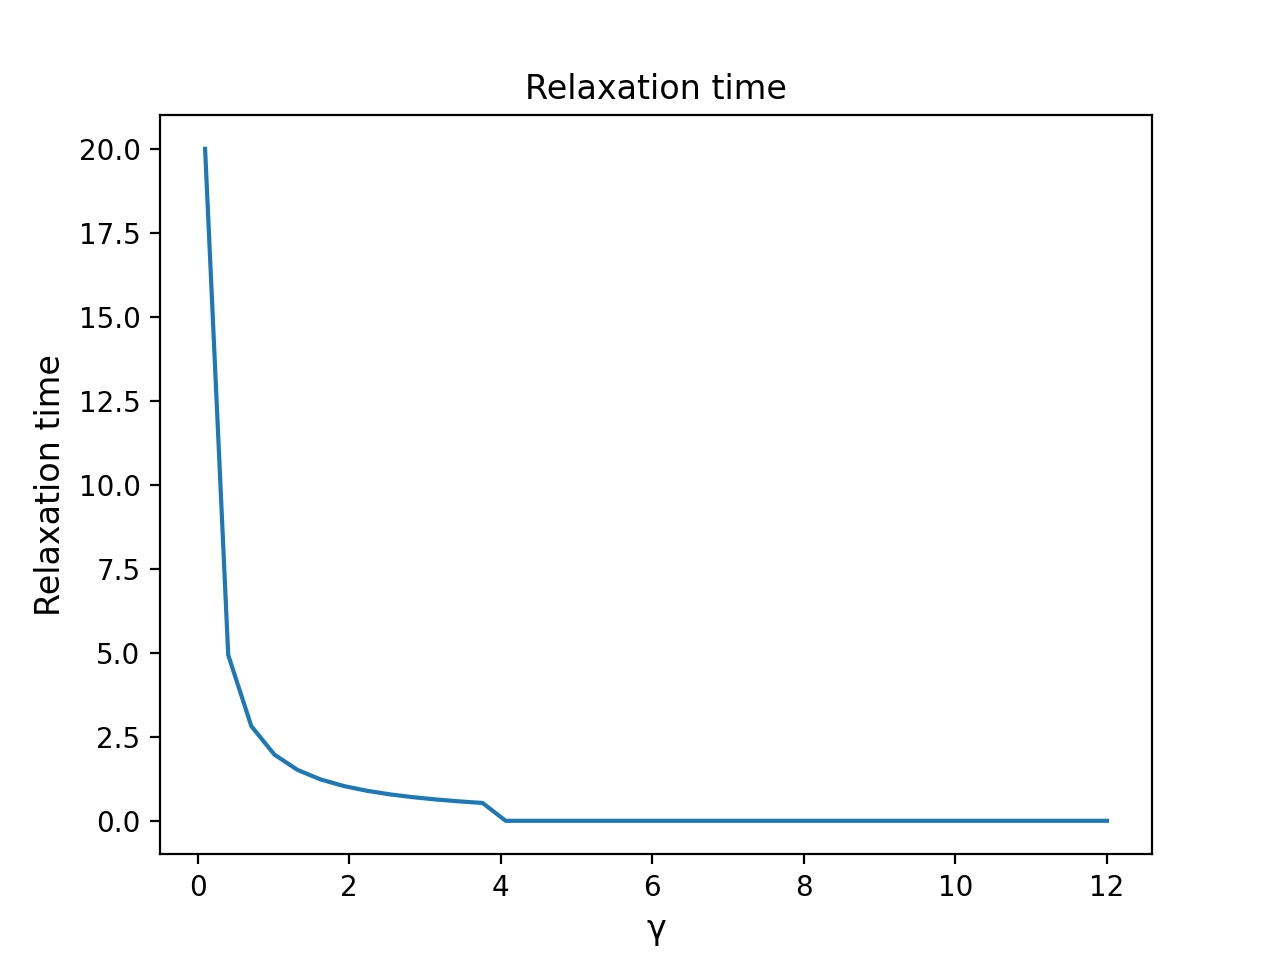
\includegraphics[width=0.45\textwidth]{RelaxationTime.jpg}
 \caption{}
\end{center}
\end{figure*}
\noindent In order to determine the relaxation time, the vertices (local maxima) of the numerical solution were plotted and fit with an exponential function in the form of: $Ae^{-kt}$. The relaxation time is subsequently calculated according to: $ T = \frac{1}{k}$. At approximately $\gamma \approx 5.9$. critical dampening occurs, as that is the inflection point of the curve.

\newpage
\section*{Project 1.4}
\subsection*{Space phase portrait for the dampened pendulum}
\begin{figure*}[ht!]
\begin{center}
    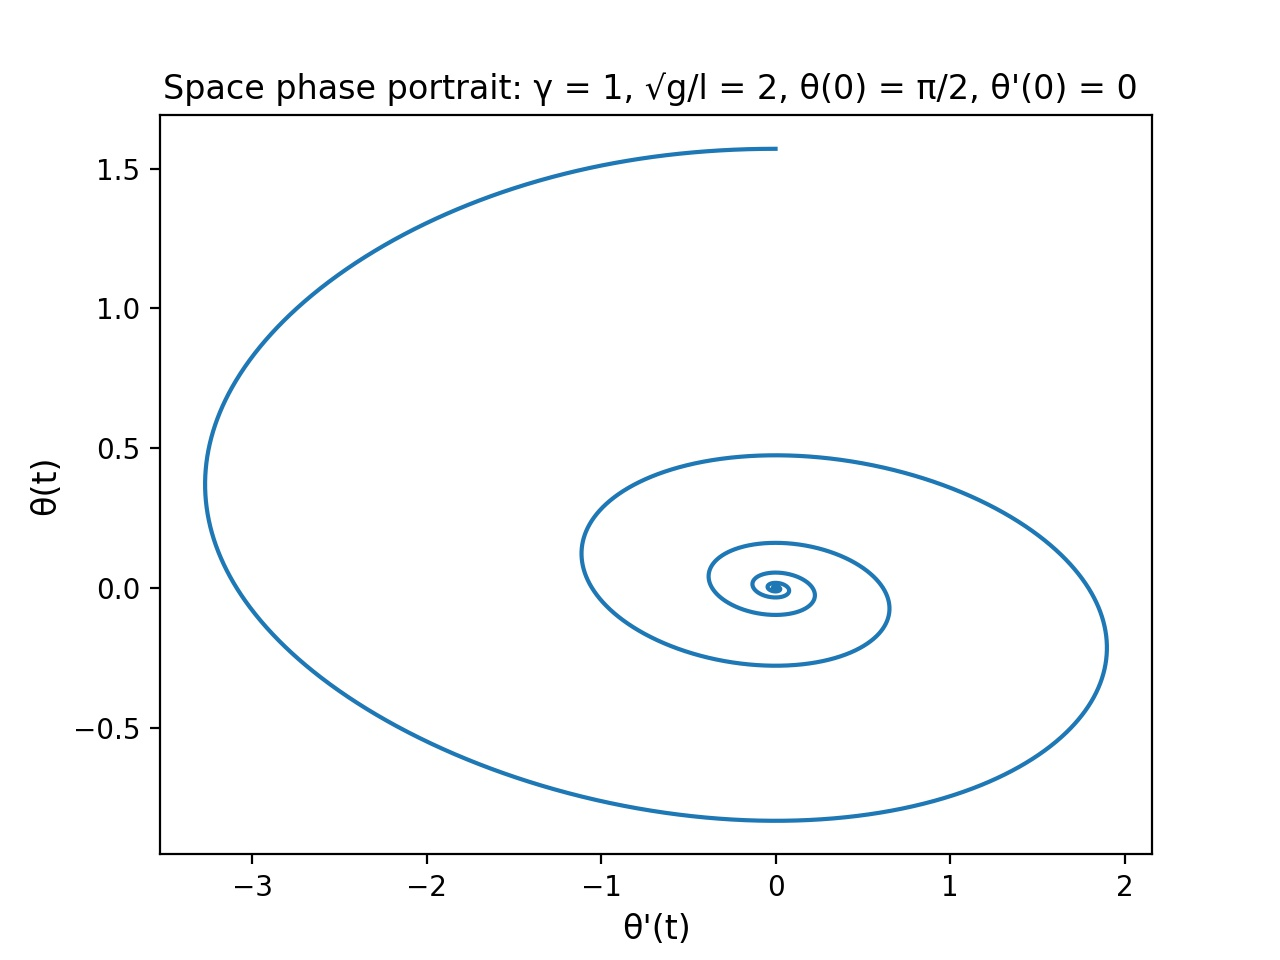
\includegraphics[width=0.5\textwidth]{SpacePhase.png}
 \caption{}
\end{center}
\end{figure*}
\noindent As ${\lim_{t \to \infty}}\theta(t) = 0$ and 
${\lim_{t \to \infty}}\theta'(t) = 0$, the spirals converge and the oscillations will eventually fade away. 
\newpage
\section*{Project 1.5}
\subsection*{The double pendulum}
Using the fourth order Runge-Kutta algorithm (with $\Delta t = 0.003$,), the generalized coordinates and momenta as function of time were plotted. Energies E = 1, 5, 10, 15 and 40 were compared, with the specified initial values. The space phase diagrams of $p_1$ versus $q_1$ and $p_2$ versus $q_2$ were also plotted. Since the latter amalgamate the time plots into concise circular orbits, they are more useful in determining the nature of the trajectories. As such the space phase diagrams are utilized for this comparison.

\begin{figure*}[ht!]
\begin{center}
   \textbf{Space phase diagrams for $p_1$ versus $q_1$}
   \subfloat[\label{genworkflow}]{%
      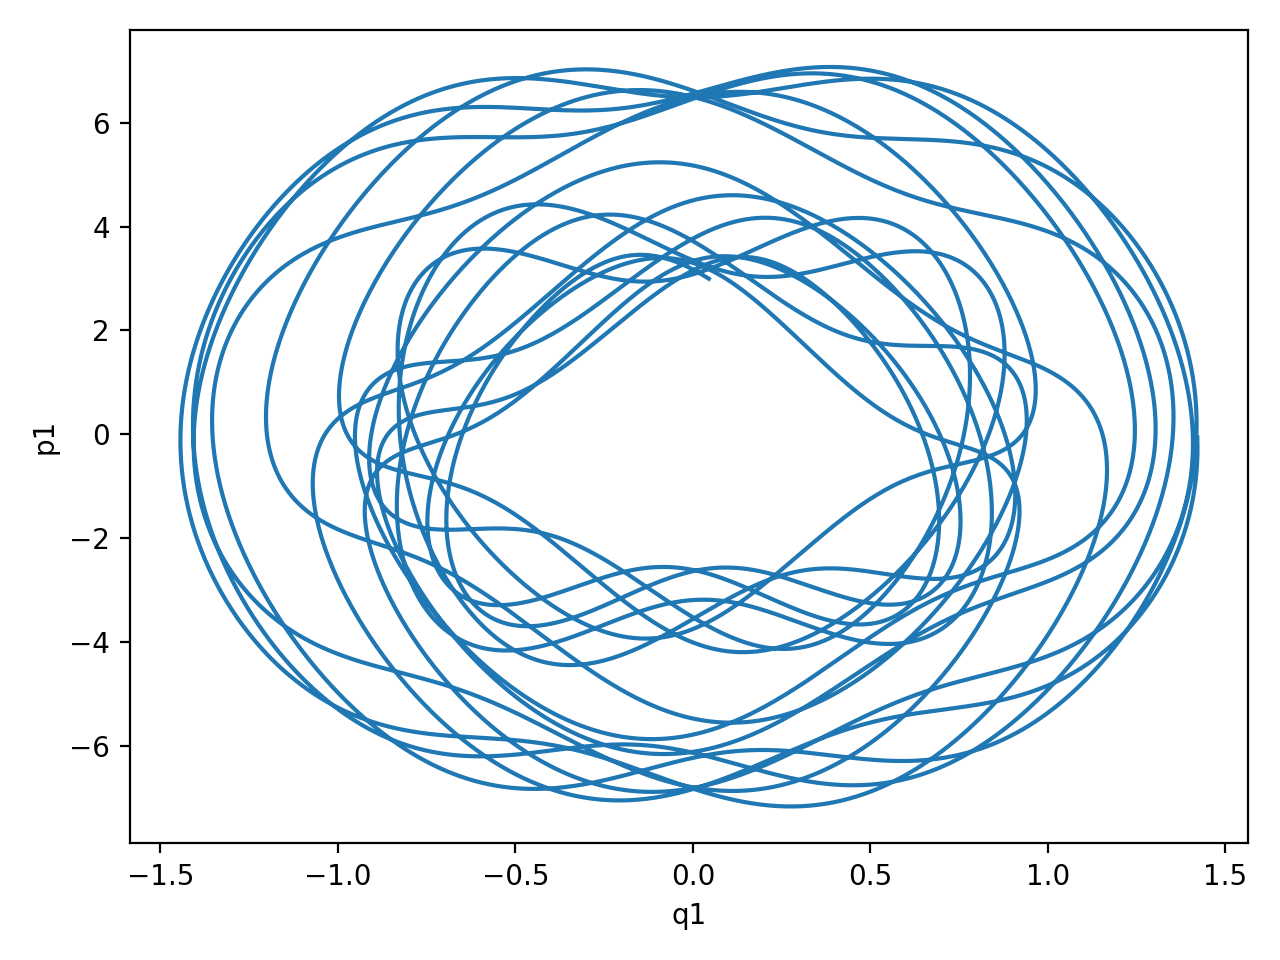
\includegraphics[ width=0.33\textwidth]{p1_E=1.jpg}}
   \subfloat[\label{pyramidprocess} ]{%
      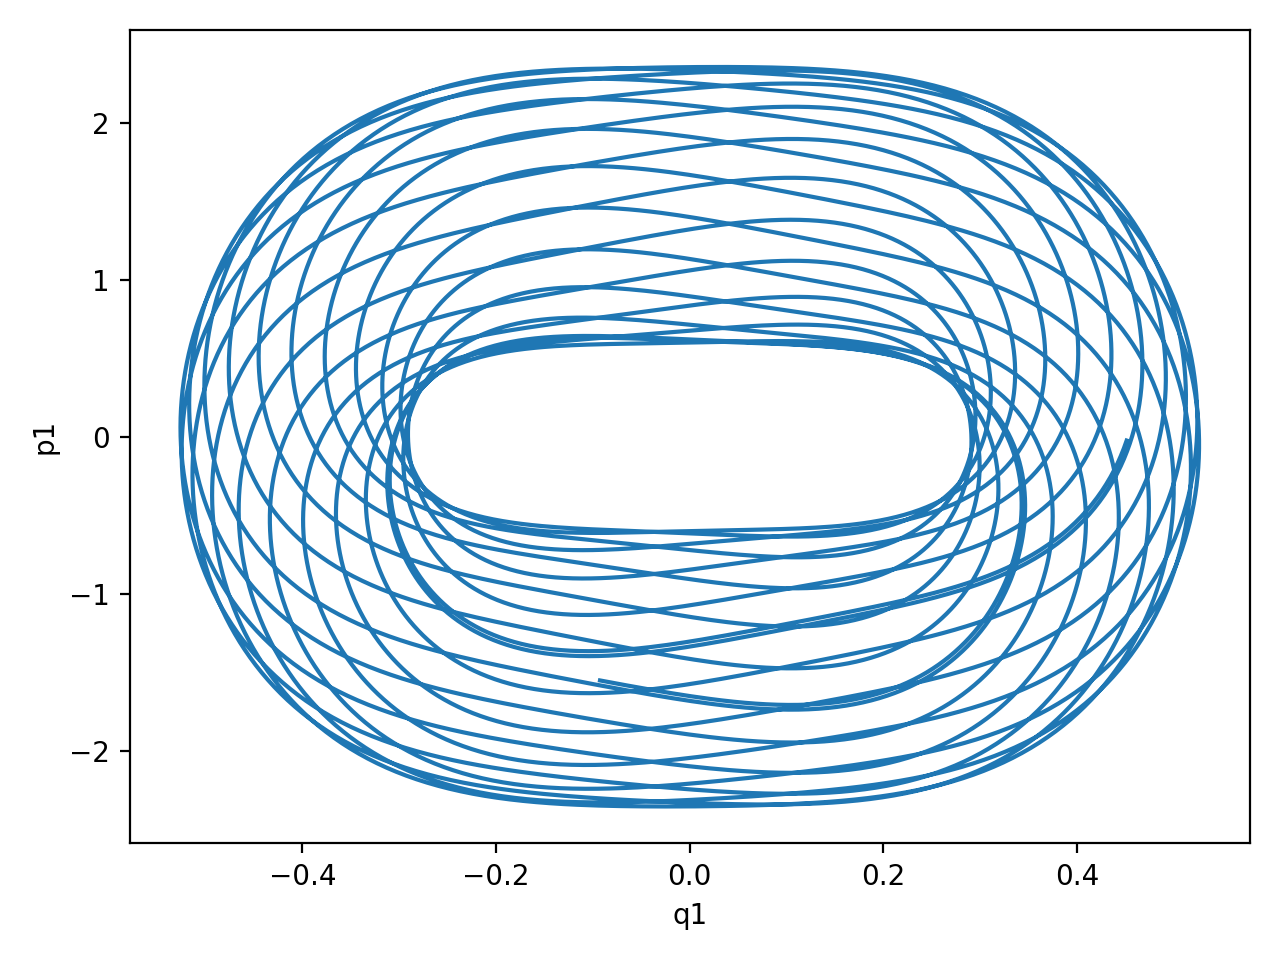
\includegraphics[ width=0.33\textwidth]{p1_E=5.jpg}}
   \subfloat[\label{mt-simtask}]{%
      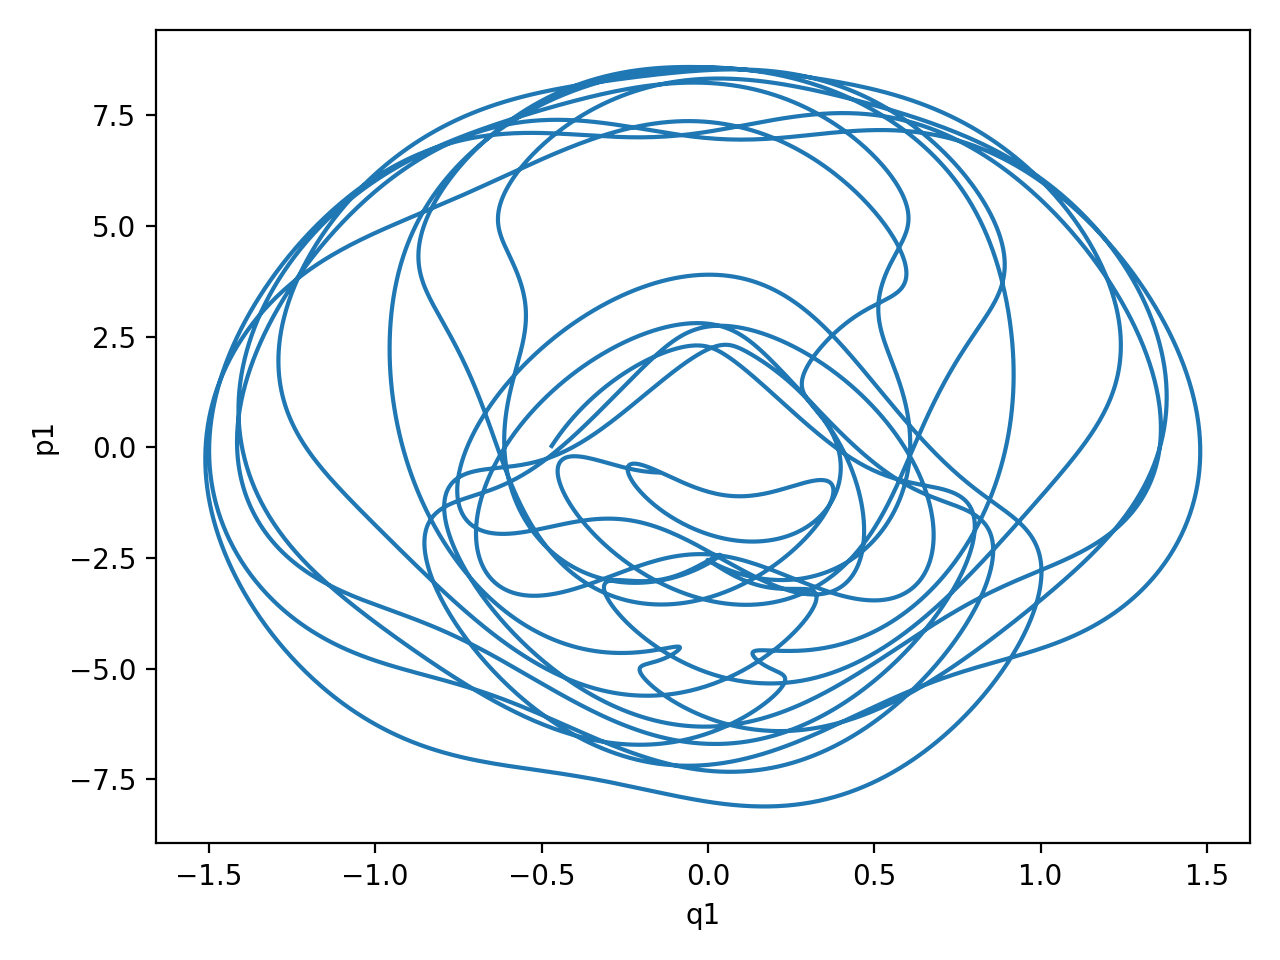
\includegraphics[ width=0.33\textwidth]{p1_E=10.jpg}}\\
   \caption{\label{workflow} 
   (a) $E = 1$; 
   (b) $E = 5$; 
   (c) $E = 10$}
\end{center}
\end{figure*}
\begin{figure*}[ht!]
\begin{center}
   \textbf{Space phase diagrams for $p_2$ versus $q_2$}
   \subfloat[\label{genworkflow}]{%
      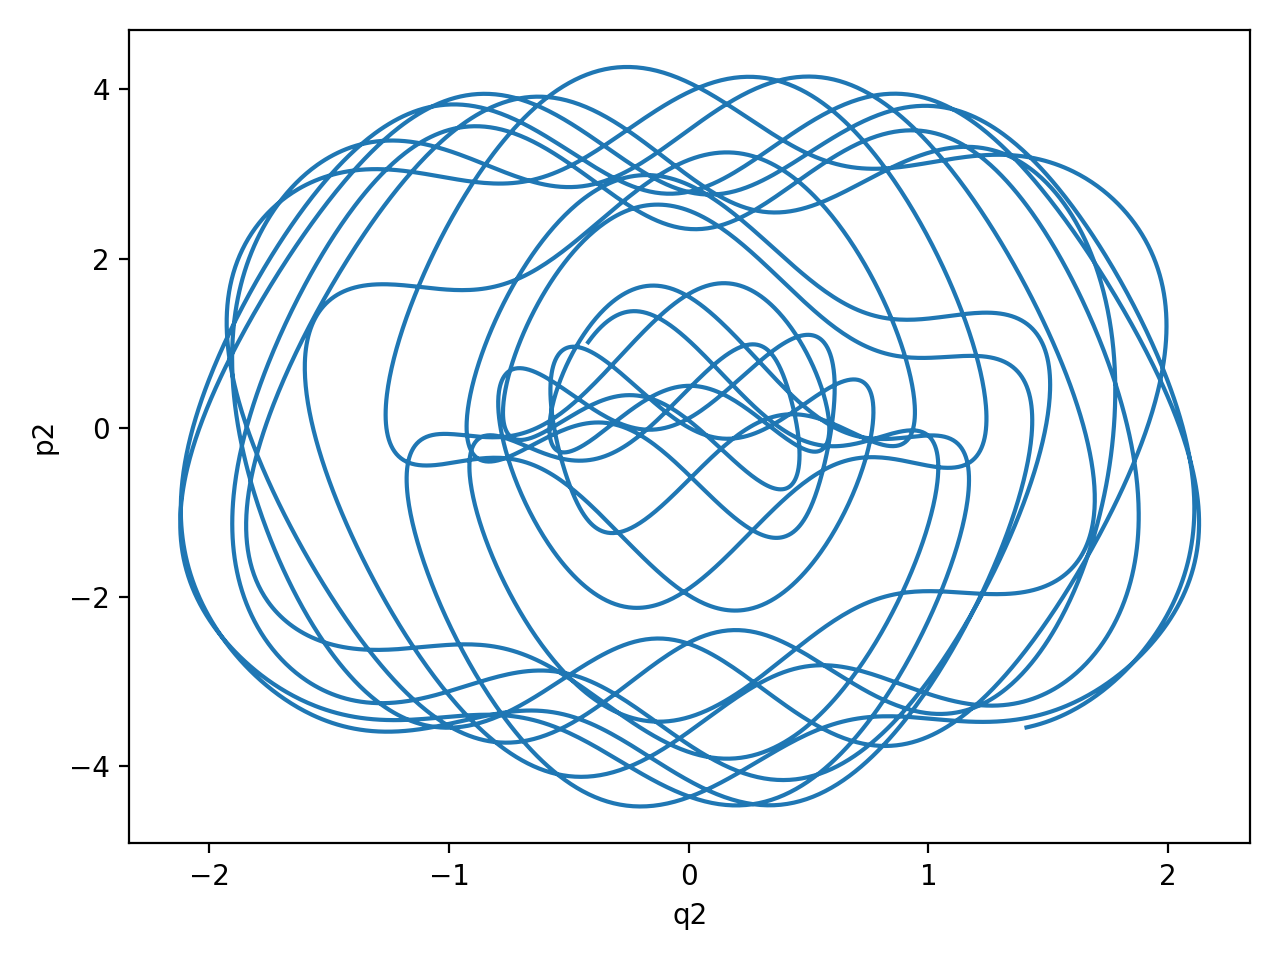
\includegraphics[ width=0.33\textwidth]{p2_E=1.jpg}}
   \subfloat[\label{pyramidprocess} ]{%
      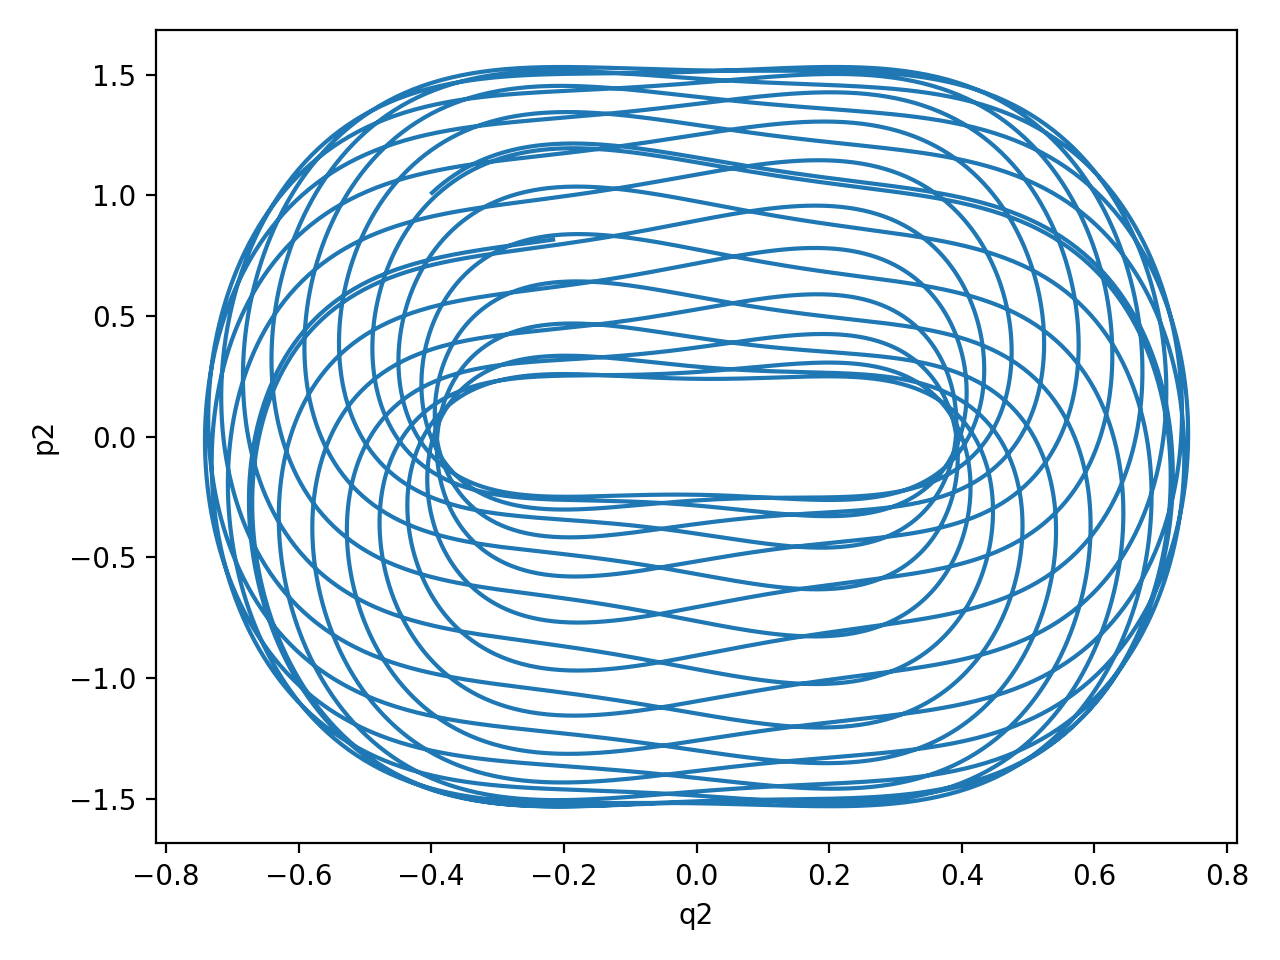
\includegraphics[ width=0.33\textwidth]{p2_E=5.jpg}}
   \subfloat[\label{mt-simtask}]{%
      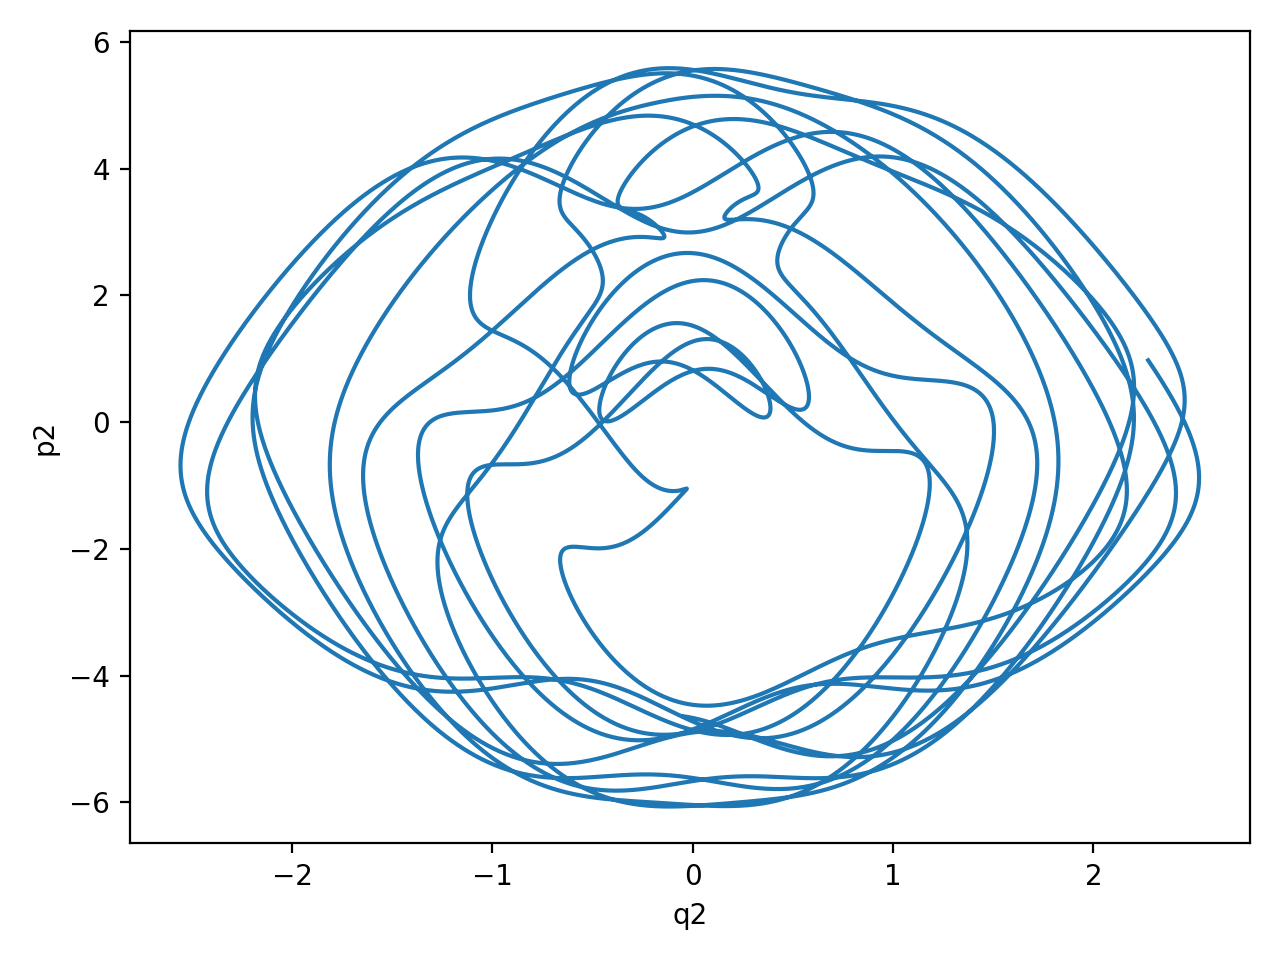
\includegraphics[ width=0.33\textwidth]{p2_E=10.jpg}}\\
   \caption{\label{workflow} 
   (a) $E = 1$; 
   (b) $E = 5$; 
   (c) $E = 10$}
\end{center}
\end{figure*}
\newpage 

\begin{figure*}[ht!]
\begin{center}
   \textbf{Space phase diagrams for $p_1$ versus $q_1$}
   \subfloat[\label{genworkflow}]{%
      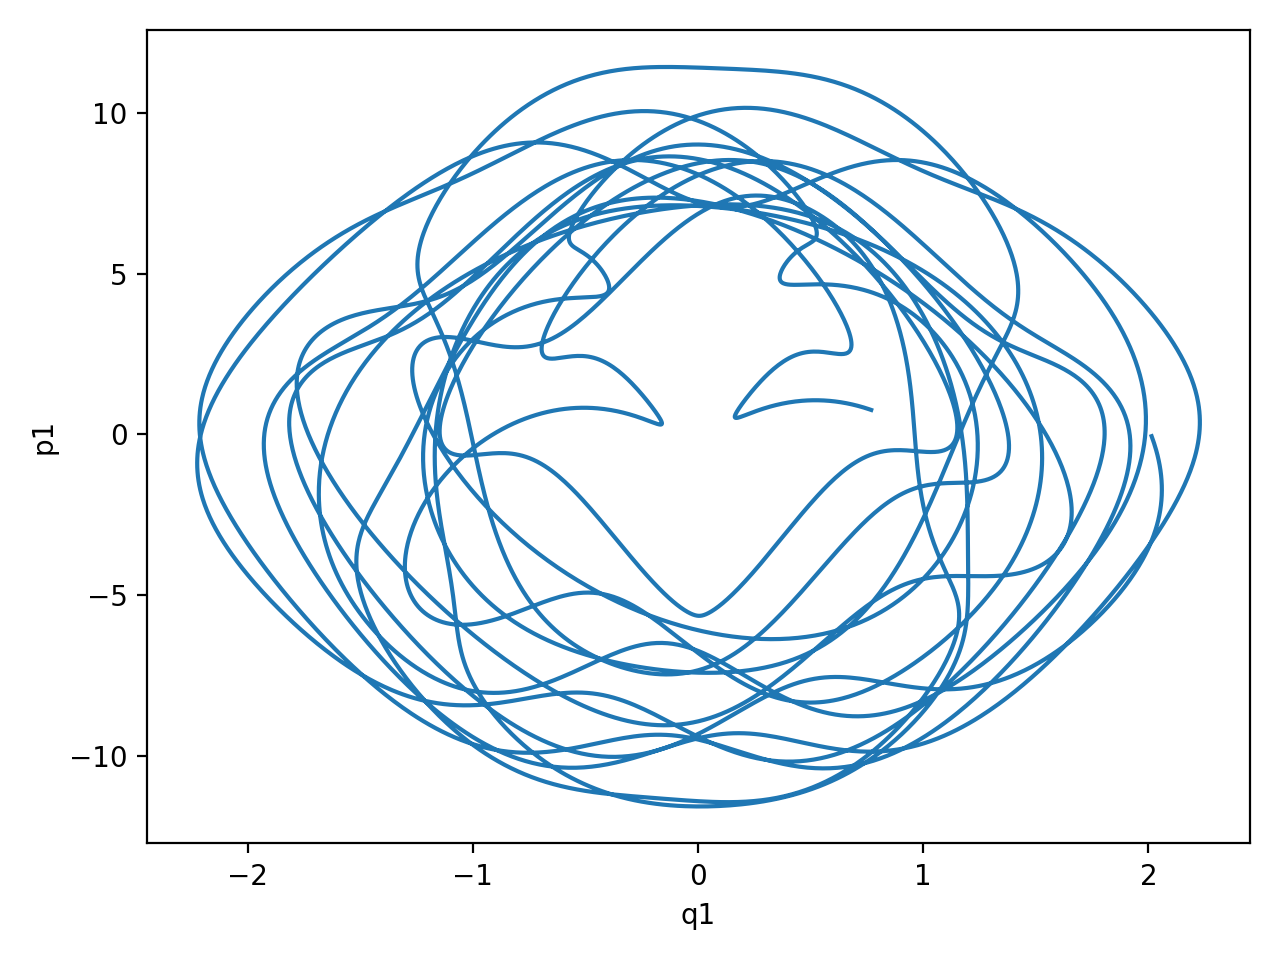
\includegraphics[ width=0.35\textwidth]{p1_E=15.jpg}}
   \subfloat[\label{pyramidprocess} ]{%
      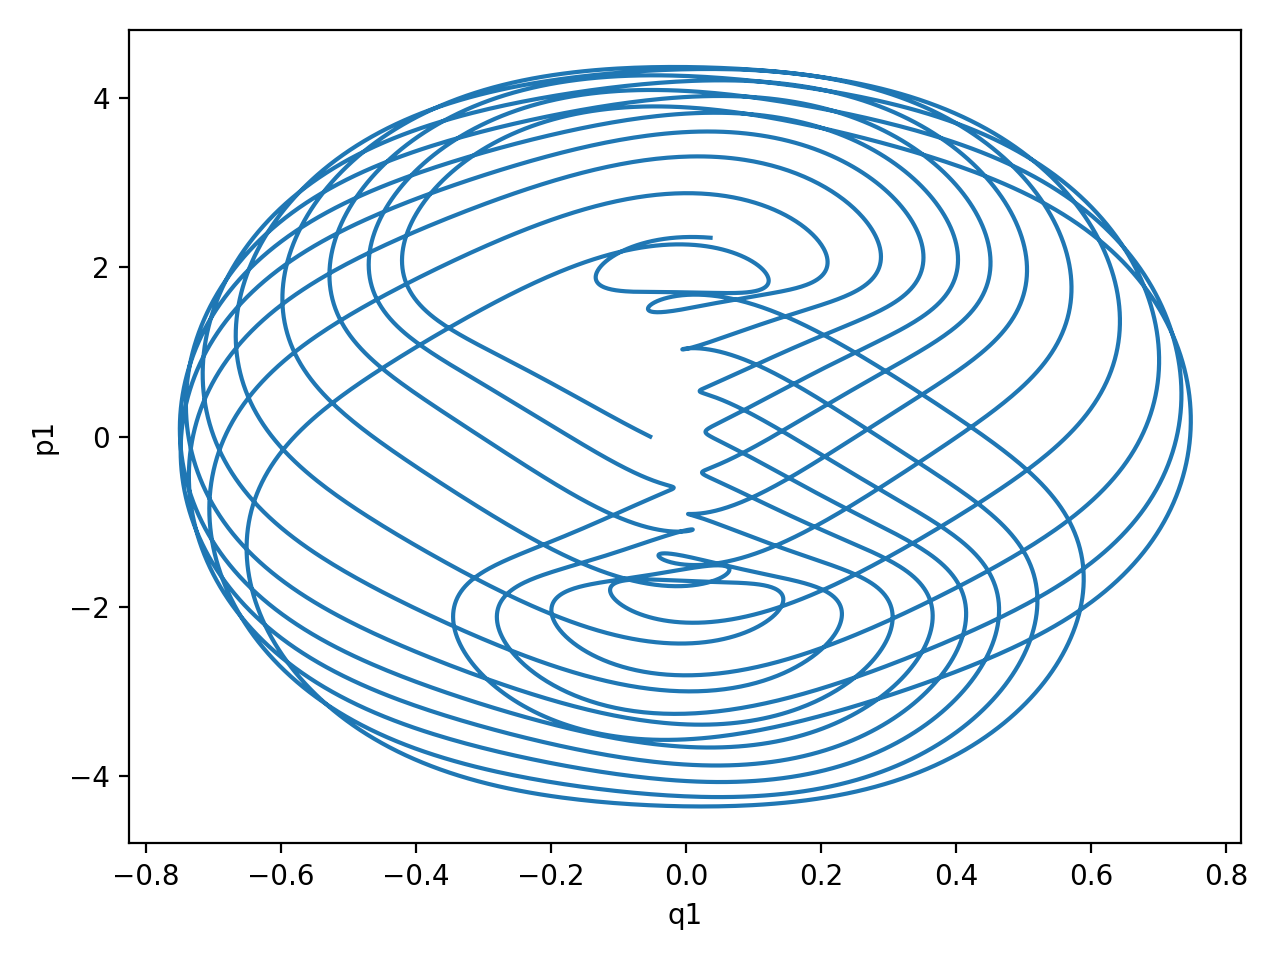
\includegraphics[ width=0.35\textwidth]{p1_E=40.jpg}}\\
   \caption{\label{workflow} 
   (a) $E = 15$; 
   (b) $E = 40$;}
\end{center}
\end{figure*}

\begin{figure*}[ht!]
\begin{center}
   \textbf{Space phase diagrams for $p_2$ versus $q_2$}
   \subfloat[\label{genworkflow}]{%
      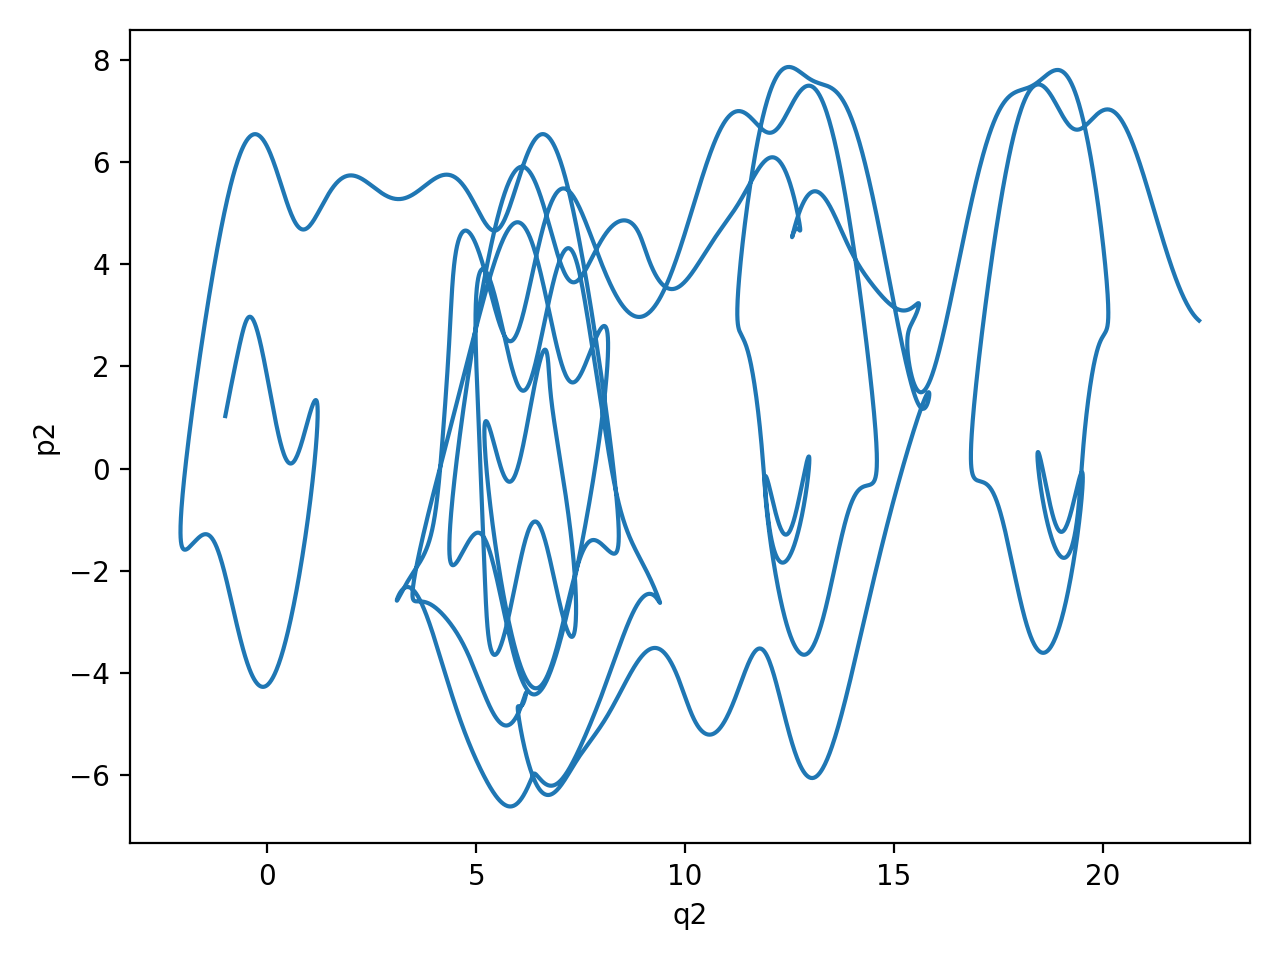
\includegraphics[ width=0.35\textwidth]{p2_E=15.jpg}}
   \subfloat[\label{pyramidprocess} ]{%
      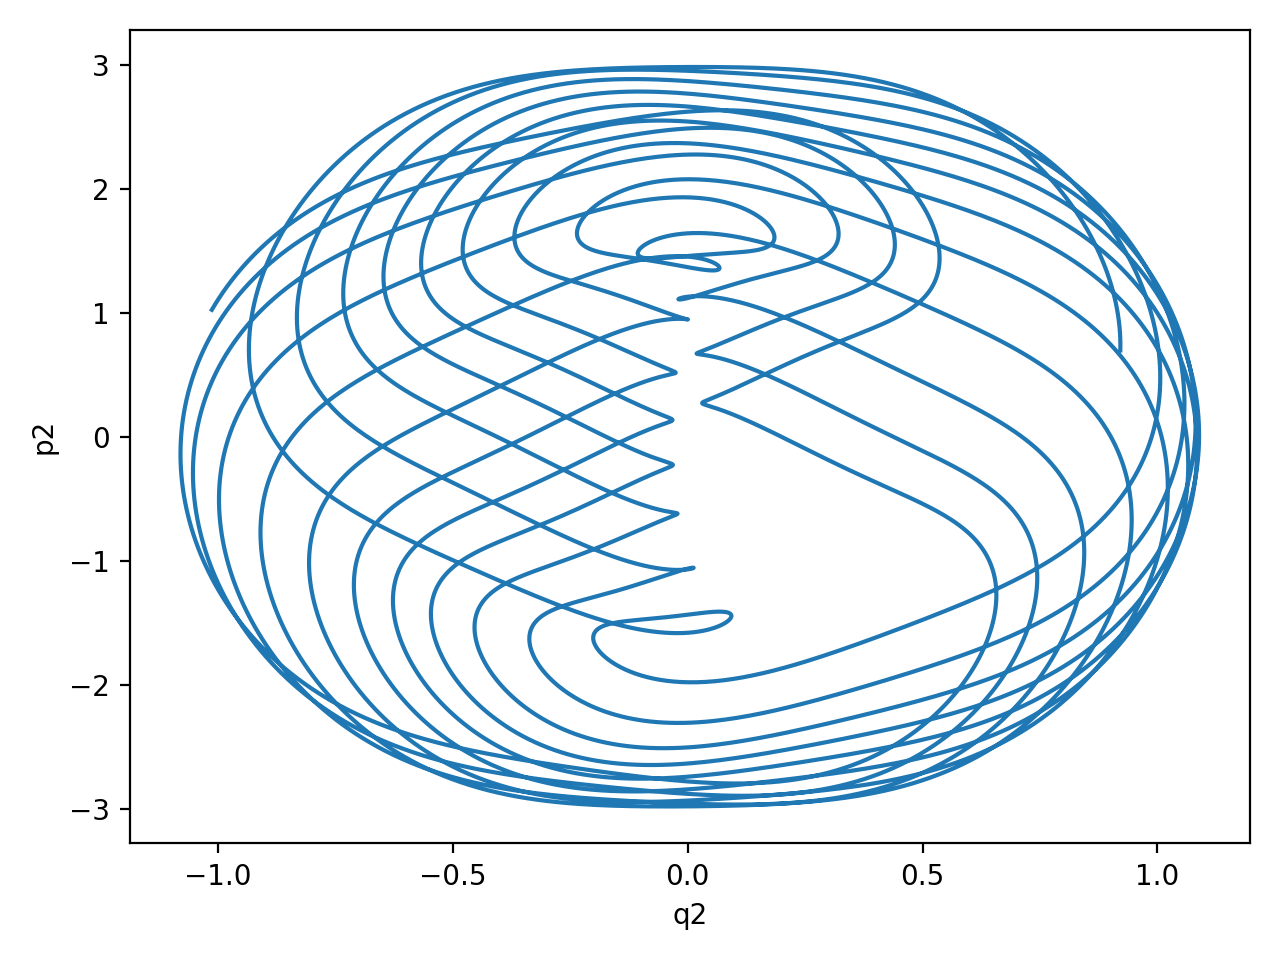
\includegraphics[ width=0.35\textwidth]{p2_E=40.jpg}}\\
   \caption{\label{workflow} 
   (a) $E = 15$; 
   (b) $E = 40$;}
\end{center}
\end{figure*}

\noindent As can be noted, the trajectories show a seemingly regular behavior for $E = 1, 5$, with $E = 5$ being the most orderly. For $E = 10$, the trajectories start regular but gradually tend toward a chaotic behavior.
For $E = 15$, it can be concluded that the $p_1-q_1$-plot shows the same semi-regular behavior as in the case of $E = 10$ while the $p_2-q_2$-plot is shown to be completely chaotic. As $E = 40$, the trajectories for the $p_2-q_2$-plot once more become regular as in the case of $E = 1$. At the meantime, $p_1-q_1$-plot tends toward a more choatic behavior.

\end{document}